%%%%%%%%%%%%%%%%%%%%%%%%%%%%%%%%%%%%%%%%%%%%%%%%%%%%%%%%%%%%%%%%%%
% The following comments were written in Portuguese, because this 
% template applies only for School of Technology at University 
% of Campinas, Brazil.
%
% Este é um modelo Latex para monografias de Trabalhos de Conclusão 
% de Curso (TCC) na graduação, monografias de Mestrado e Teses de 
% doutorado da Faculdade de Tecnologia (FT) da Universidade 
% Estadual de Campinas (UNICAMP).
%
% Esse modelo e seu respectivo arquivo de classe de documento 
% foram adaptado do modelo de teses e dissertações do 
% Instituto de Computação da UNICAMP.
%
% Autor: André Leon Sampaio Gradvohl, Dr.
% Email:        gradvohl@ft.unicamp.br
% Lattes CV:    http://lattes.cnpq.br/9343261628675642
% ORCID:        0000-0002-6520-9740
% 
% Última versão: 24/Março/2019
%
% Adições/Alterações nesta última versão 
% - Alteração da fonte padrão (times) para fonte libertine, mais 
%   adequada do que a Times New Roman para teses, mas ainda
%   compatível com a times.
% - Adição de comandos para abreviações especiais, e.g., i.e. e
%   p.ex., respectivamente \eg , \ie , \pex
% - Adição do pacote booktabs para tabelas.
% - Ajustes nas referências bibliográficas de acordo com a norma 
%   ABNT NBR 6023 de 14/11/2018.
%%%%%%%%%%%%%%%%%%%%%%%%%%%%%%%%%%%%%%%%%%%%%%%%%%%%%%%%%%%%%%%%%%
%
% Escolha: Portugues ou Ingles ou Espanhol.
% Para a versão final do texto, acrescente a palavra "Final",
% como na segunda linha abaixo da próxima.
%\documentclass[Portugues]{tese-FT}
\documentclass[Portugues,Final]{tese-FT}
%\documentclass[Ingles]{tese-FT}
%\documentclass[Espanhol,Final]{tese-FT}

%Adicione seu arquivo com as referências bibliográficas
\addbibresource{bibliografia.bib}

%O pacote a seguir gera um dummy text. Elimine a linha quando
% for editar seu texto.
%\usepackage{lipsum}
%%%%%%%%%%%%%%%%%%%%%%%%%%%%%
%User packages

\usepackage{soul}
\usepackage{cancel}
\newcommand\tab[1][1cm]{\hspace*{#1}}
\usepackage{amsmath}
\usepackage{minted}
\usepackage{booktabs}
\usepackage{cancel}
\usepackage{enumitem}
\usepackage{subfig}
%\usepackage[switch, modulo]{lineno}
\usepackage{circuitikz}
\usepackage{indentfirst}
\usetikzlibrary{shapes,arrows,positioning,calc}
\usetikzlibrary{decorations}
\usepackage{pgfplotstable}
\usepackage{pgfplots}
\usepackage{caption}
\usepackage{subcaption}

% Adicione o pacote a seguir, se seu texto tiver uma lista de 
% símbolos. Não confunda com a lista de abreviaturas.
%\usepackage[symbols,nogroupskip,sort=none]{glossaries-extra}

\begin{document}

% Escolha entre autor ou autora:
\autor{Pedro Henrique Neves dos Santos}
%\autora{Nome da Autora}

% Sempre deve haver um título em português:
\titulo{Proposta de tema de mestrado\\ Conversor CC-CC com topologias baseadas em transistores tipo GaN}

% Se a língua for o inglês ou o espanhol defina:
%\title{The Dissertation or Thesis Title in English or Spanish for FT}

% Escolha entre orientador ou orientadora e inclua os títulos:
\orientador{Prof. Dr. Ernesto Ruppert Filho}
%\orientadora{Profa. Dra. Nome da Orientadora}

% Escolha entre coorientador ou coorientadora, se houver, 
% e inclua os títulos:
%\coorientador{Prof. Dr. Eng. Lic. Nome do Co-Orientador}
%\coorientadora{Prof. Dra. Eng. Lic. Nome da Co-Orientadora}

% Escolha entre uma das quatro opções a seguir (comente as demais):
%\bsi         % para Trabalho de Conclusão de Curso em BSI
%\tads       % para Trabalho de Conclusão de Curso em TADS
%\qualificacaoMestrado  % Para textos de qualificação de mestrado.
%\qualificacaoDoutorado % Para textos de qualificação de doutorado.
\mestrado   % para Dissertação de Mestrado em Tecnologia
%\doutorado  % para Tese de Doutorado em Tecnologia

%Defina a área de concentração. Se for TCC, deixe comentado
\areaConcentracao{Sistemas de Informação e Comunicação}
%\areaConcentracao{Ambiente}
%\areaConcentracao{Ciência dos Materiais}

% Se houve cotutela, defina:
%\cotutela{Universidade Nova de Plutão}

%Defina a data da defesa no formato {Dia}{Mês}{Ano}
\datadadefesa{13}{05}{2021}

% Para a versão final defina:
% Repita o nome do Orientador(a) no primeiro avaliador
%\avaliadorA{Prof. Dr. Nome do Orientador}{FT/UNICAMP}
%\avaliadorB{Profa. Dra. Segunda Avaliadora}{Instituição da segunda avaliadora}
\avaliadorC{Dr. Terceiro Avaliador}{Instituição do terceiro avaliador}
% \avaliadorD{Prof. Dr. Quarto Avaliador}{Instituição do quarto avaliador}
% \avaliadorE{Prof. Dr. Quinto Avaliador}{Instituição do quinto avaliador}
% \avaliadorF{Prof. Dr. Sexto Avaliador}{Instituição do sexto avaliador}
% \avaliadorG{Prof. Dr. Sétimo Avaliador}{Instituição do sétimo avaliador}
% \avaliadorH{Prof. Dr. Oitavo Avaliador}{Instituição do oitavo avaliador}


% Para incluir a ficha catalográfica em PDF na versão final, 
% copie o arquivo PDF, descomente e ajuste a linha a seguir:
%\fichacatalografica{arquivo.pdf}

% Este comando deve ficar aqui:
\paginasiniciais
% Sempre deve haver um resumo em português:
%\begin{resumo}

%Primeiro trabalho apresentado \`a disciplina IT306.\\\\\
%Neste quarto trabalho, será abordado 
%\href{https://github.com/phneves/ElectricPowerSystemsAnalysisTools}{https://github.com/phneves/ElectricPowerSystemsAnalysisTools}



%\end{resumo}


% A lista de símbolos é opcional. Não confunda a lisa de símbolos
% com a lista de abreviaturas.
%\prefacesection{Lista de Símbolos}

% Coloque o símbolo na primeira coluna e a 
% descrição na segunda coluna. Use descrições
% rápidas.

\begin{table}[!ht]
  \begin{tabular}{p{3cm}l}
	$NB$        & N\'umero de Barras \\
	$k$       & Inteiro entre 1 e $NB$\\
	$m$        & N\'umero de Barras \\
	$\in$       & Inteiro entre 1 e $NB$\\
	$\kappa$        & Conjunto formado pela barra $k$ e todas as barras $m$ conectadas ela \\
	$G_{km}$       & Inteiro entre 1 e $NB$\\
	$B_{km}$        & N\'umero de Barras \\
	$k$       & Inteiro entre 1 e $NB$\\
	
	$c$       & Descrição do símbolo $c$ 
  \end{tabular}
\end{table}

% A lista de abreviações e siglas vem a seguir.
% Dê uma olhada no pacote nomencl para ver os comandos para 
% adicionar abreviações e siglas no texto.
\renewcommand{\nomname}{Lista de Abreviações e Siglas}
\printnomenclature[3cm]


% O sumário vem aqui:
\tableofcontents
\fimdaspaginasiniciais


% O corpo da dissertação ou tese começa aqui:
%
% O comando a seguir inclui o arquivo introducao.tex
% que contém o capítulo de Introdução. 
% Detalhe: não precisa incluir a extensão .tex
%\include{introducao}

%\linenumbers
\chapter{Objetivos do trabalho}
\label{chapterObjetivos}
\section{Transistores \textit{wide bandgap}: GaN}
Segundo a \textit{World Semiconductor Trade Statistics}, cada pessoa no planeta comprou uma média de 111 chips ou circuitos integrados (ICs) em 2016. O uso desses dispositivos semicondutores está crescendo cinco vezes a taxa de crescimento da população humana \cite{Sameer}. Natural que haja uma busca por dispositivos que possibilitem maior densidade de transistores, bem como menor dissipação de energia na forma de calor. Transistores de Nitreto de Gálio e Carbeto de Silício vem se mostrando como alternativa ao cenário atual, com Silício. No caso do Nitreto de Galio, são bons chaveadores em alta frequência além baixa resistência quando ligados \cite{lidow_rooij_strydom_reusch_glaser_2020}. 
\par Assim, o emprego de transistores GaN apresenta grande vantagem quando inserido em aplicações sensíveis à eficiencia energética, especialmente como dispositivos portáteis ou à bateria, além de dar mais flexibilidade ao projeto, uma vez que ao chavearem em mais alta frequência, elementos magnéticos menores podem ser usados nos projetos de fontes chaveadas, por exemplo.  
\par Neste trabalho, transistores do tipo GaN serão empregados em um sistema solar fotovoltaico de pequeno porte para alimentação de uma bateria Li-Ion(18650) como na figura \ref{FigDiagBlocoSistema}.
\par Os capitulos \ref{chapterObjetivos} e \ref{chapterRevisao} contextualizam e definem modelos matemáticos necessários para aplicação do transistor tipo GaN em fontes chaveadas, nos capítulos \ref{chapterMetodologia} será apresentado a simulação computacional dos modelos descritos nos capitulos anteriores. Os resultados parciais dos blocos já simulados e analises já encaminhadas se encontam no capitulo \ref{chapterResultados}.

\begin{figure}[H]
\caption{Diagrama de blocos} 
\begin{center}
\begin{circuitikz}
%Coluna,Linha
%(0,0) botton left

\draw %painel solar
    (0,0)   to [short,i=] (3,0)
    (3,0)   to [short] (3,3)
    (3,3)   to [short] (0,3)
    (0,3)   to [short] (0,0)
    (1.5,1.5) node[]{Painel Fotovolt.};

\draw %MPPT
    (3.5,-1)   to [short,i=] (5.5,-1)
    (5.5,-1)   to [short,i=] (5.5,-2)
    (5.5,-2)   to [short,i=] (3.5,-2)
    (3.5,-2)   to [short,i=] (3.5,-1)
    (4.5,-1.5) node[]{MPPT};

\draw %buck
    (6,0)   to [short,i=] (9,0)
    (9,0)   to [short] (9,3)
    (9,3)   to [short] (6,3)
    (6,3)   to [short] (6,0)
    (7.5,1.5) node[]{Buck};

\draw %Controle
    (6,-1)   to [short,i=] (9,-1)
    (9,-1)   to [short,i=] (9,-2)
    (9,-2)   to [short,i=] (6,-2)
    (6,-2)   to [short,i=] (6,-1)
    (7.5,-1.5) node[]{Controle};

\draw %bateria   
    (12,2.5)   to [battery,i=] (12,-1)
    node[ground]{};

\draw %Connections    
    (3,2.5)   to [ammeter] (6,2.5)
    (3,0.5)   to [short] (6,0.5)
    (3.5,0.5) to [voltmeter,*-*] (3.5,2.5)
    
    (11,-1) to [voltmeter,-*] (11,2.5)
    (11,-1) node[ground]{}
    (9,2.5)   to [ammeter] (11,2.5)
    (11,2.5)   to [short] (12,2.5)
    
    (4.5,2.1) to [short] (4.5,-1)
    (4.1,1.5) to [short] (4.1,-1)
    (3.9,1.5)   to [short] (4.1,1.5)
    
    (5.5,-1.5)   to [short] (6,-1.5)
    (7.5,-1)   to [short] (7.5,0)
    ;
\end{circuitikz}
\end{center}
\label{FigDiagBlocoSistema}
\end{figure}
%\begin{figure}[H]
%\caption{Diagrama de bloco}
% \centering % para centralizarmos a figura
%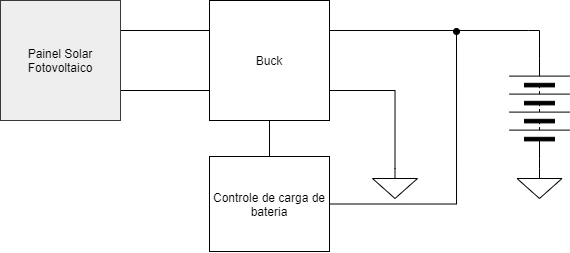
\includegraphics[width=6cm]{figuras/DiagramaBlocos.png} 
%\label{FigDiagBlocoSistema}
%\end{figure}


\section{Paineis solares fotovoltáicos}
%REESCREVER - CÓPIA DO ARTIGO DO BRANDAO/VILALLVA - trocar o título talvez
%\par A escolha do sistema utilizado passa pela necessidade de acesso a energia em comunidades remotas e carentes, que em grande parte das vezes não conseguem acesso nem ao mais basico acesso à energia elétrica. Isso limita a rotina, o convívio social e ainda expõe esses brasileiros a diversos riscos, como ataques de animais. Além disso, o uso de lamparinas para suprir a ausência de eletricidade afeta a saúde da população e pode causar incêndios nas casas.
%\par Diante deste cenário, um sistema de energia solar de pequeno porte, que carregue uma bateria é vital para manter iluminação e para carregar pequenos dispositivos, garantindo assim aumento na qualidade de vida como um todo. 
%\par A associação Pisco de Luz \cite{pisco} faz um trabalho importante para alterar esta realidade. 
%\par O sistema solar fotovoltaico é composto por um painel solar fotovoltaico, conversores chaveados e, podem ou não ser conectados à rede elétrica.\\
%...
%Esperar livro do Marcelo Vilalva.
%\par Majoritariamente, a fonte de energia do nosso planeta é solar, seja na forma de luz ou calor. \cite{Villalva}.
%\par As fontes de energias renováveis vêm desempenhando um importante papel no cenário mundial, principalmente devido à crescente preocupação com
%o meio ambiente – efeito estufa e aquecimento global– e ao contínuo aumento da demanda energética.Neste contexto, os sistemas de geração distribuída
%despertam grande interesse, pois podem utilizar diversos tipos de fontes primárias de energia, podem ser instalados próximos às cargas e atenuam as necessidades imediatas dos governos em realizar investimentos onerosos na matriz energética (XuWei,2009, Pomílio, 2011).
%\par Um conjunto controlado de sistemas de geração distribuída e cargas locais pode ser denominado microrrede. Uma microrrede pode ser entendida como um pequeno sistema de energia elétrica controlável que pode, entre outras coisas, auxiliar as concessionárias no processo de despacho de energia,redução das perdas no processo de transmissão e correção de afundamentos de tensão. Pode ainda ser desconectado automaticamente do sistema de distribuição em casos de faltas elétricas ou intencionalmente, de acordo com a vontade do usuário (Lasseter, 2007 e Kroposki, 2008). 
%\par A energia fotovoltaica se destaca das outras fontes renováveis e limpas principalmente pelo fato de poder ser instalada rapidamente em comércios e
%residências, além de ser silenciosa e inesgotável (Barker, 2005). As principais desvantagens dos sistemas fotovoltaicos são a baixa eficiência dos módulos comerciais de silício cristalino, que atualmente está em torno de 15\% e, o elevado custo de instalação, devido aos módulos e aos conversores eletrônicos.
%\par Os sistemas de geração distribuída podem operar como sistemas autônomos e/ou sistemas interligados à rede elétrica. O primeiro tipo é fundamental para o processo de inclusão social, fornecendo energia elétrica às propriedades que não têm acesso ao sistema de distribuição. O segundo tipo, que pode ser usado em zonas urbanas e densamente povoadas, é mais interessante por sua contribuição ao sistema elétrico nacional, pois pode aliviar os picos de demanda e as linhas de transmissão e de distribuição, que já operam em sua capacidade máxima \cite{BrandaoVilallalva}.
\chapter{Revisão bibliográfica}
\label{chapterRevisao}
\section{Transistores em circuitos de potência}
\label{sectionCap2transistores}
\subsection{Transistores de potência baseados em Silício}
Os transistores de potência baseados em silício, tiveram sua eficiência e o custo do gerenciamento de energia melhorado continuamente nas ultimas decadas. Inovações em estruturas do transistor acompanharam a crescente necessidade de equipamentos eletrônicos em nossas vidas diárias. No entanto, a taxa de melhoria diminuiu bastante, uma vez que, assintoticamente, se aproxima de seus limites teóricos. \cite{lidow_rooij_strydom_reusch_glaser_2020}

\subsection{Transistor baseados em Nitreto de Gálio (GaN)}
Dispositivos baseados em Nitreto de Gálio (GaN) apareceram pela primeira vez em cerca de 2004, como transistores de radiofrequência (RF) feitos pela Eudyna Corporation do Japão. Usando GaN em substratos de carbeto de silício (SiC), a Eudyna produziu transistores projetados para o mercado de RF, com sucesso \cite{Alex}. Porém, não só do ponto de vista de RF há vantagens em utilizar GaN, há vantagens também em eletrônica de potência. As caracteristicas dos dispositivos baseados em Nitreto de Gálio podem ser vistas na comparação da Tabela \ref{t_materiais}.

\begin{table}[!htb]
\centering
\caption{Comparação entre propriedades dos materiais \cite{lidow_rooij_strydom_reusch_glaser_2020}}
\begin{tabular}{lllll}
\hline
Parâmetro           &                & Si    & SiC   & GaN \\ \hline
Banda de Gap $E_g$& $(eV)$             & 1,12  & 3,39  & 3,26\\
Campo Elétrico crítico $E_{Crit}$ &$(MV/cm)$   & 0,23  & 3,3   & 2,2\\
Mobilidade dos elétrons $\mu_n$ &$(cm^2/V.s)$& 1400  & 1500  & 950\\
Permissividade $\varepsilon_r$ &     & 11,8  & 9     & 9,7\\
Condutividade térmica $\lambda$& $(W/cm.K)$     & 1,5   & 1,3   & 3,8\\ \hline
\end{tabular}
\label{t_materiais}
\end{table}

\subsubsection{Banda de Gap $(E_g)$}
A banda de Gap de um semicondutor está relacionado à força das ligações químicas entre os átomos na rede. Essas ligações mais fortes significam que é mais difícil para um elétron saltar de um nível para o próximo. Entre as muitas consequências estão correntes de fuga intrínsecas mais baixas e maiores temperaturas de operação para semicondutores de gap maior. Com base nos dados da Tabela \ref{t_materiais}, GaN e SiC têm banda de Gap maiores do que o silício. \cite{lidow_rooij_strydom_reusch_glaser_2020}

\subsubsection{Resistência quando ligado $(R_{DS_{(on)}})$}
\par A resistência teórica, em Ohms ($\Omega$), será dada pela equação \ref{RdsOn}. \cite{lidow_rooij_strydom_reusch_glaser_2020}
\begin{equation}
    R_{DS_{(on)}} = \frac{W_{drift}}{q.\mu_n .N_D}
    \label{RdsOn}
\end{equation}
\par A resistência, quando relacionada com o Campo Elétrico Crítico $(E_g)$ será dada por \ref{RdsOnEg}. \cite{lidow_rooij_strydom_reusch_glaser_2020}
\begin{equation}
    R_{DS_{(on)}} = \frac{4.V^2_{BR}}{\varepsilon_o .\varepsilon_r . E^3_{crit}}
    \label{RdsOnEg}
\end{equation}
\par A equação dada por \ref{RdsOnEg} está representada no gráfico da Figura \ref{FigRDSon}.
\begin{figure}[H]
\caption{Resistência $R_{DS_(on)}$ vs capacidade de bloquear tensão para dispositivos Si, SiC, and GaN \cite{lidow_rooij_strydom_reusch_glaser_2020}}
 \centering % para centralizarmos a figura
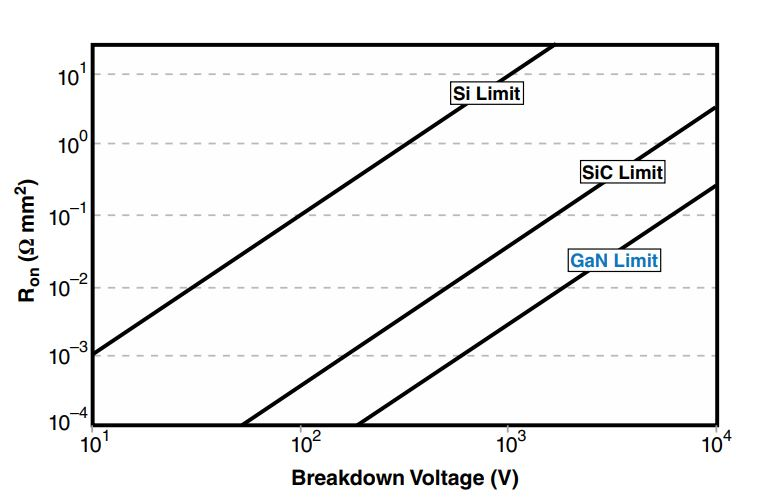
\includegraphics[width=10cm]{figuras/5.JPG} 
\label{FigRDSon}
\end{figure}
\noindent Junto com a baixa resistência $R_{DS_(on)}$, há o benefício de conseguir trabalhar em frequências mais altas que IGBTs com potências relativamente altas, como mostra a Figura \ref{FigComparison}. 
\begin{figure}[H]
\caption{Potência vs Frequência. \cite{Sameer}}
 \centering % para centralizarmos a figura
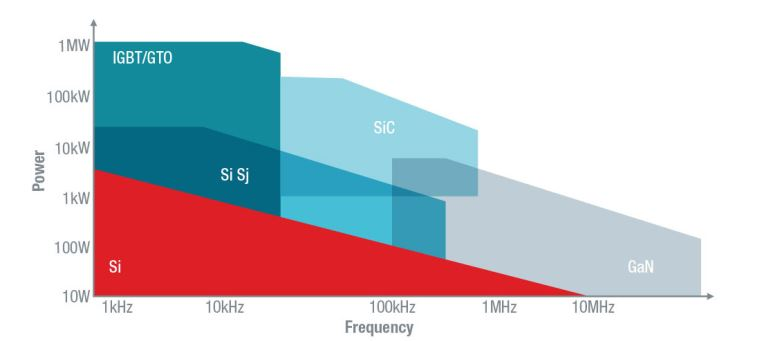
\includegraphics[width=14cm]{figuras/6.JPG} 
\label{FigComparison}
\end{figure}

%%%%%%%%%%%%%%%%%%%%%%%%%%%%%%%%%%%%%%%%%%%%%%%%%%%%%%%%%%%%%%%%%%%%%%%%%%%%%%%%%%%%%%%%%%%%%%%%%%%%%%%%%%%%%%%%
%%%%%%%%%%%%%%%%%%%%%%%%%%%%%%%%%%%%%%%%%%%%%%%%%%%%%%%%%%%%%%%%%%%%%%%%%%%%%%%%%%%%%%%%%%%%%%%%%%%%%%%%%%%%%%%%
%%%%%%%%%%%%%%%%%%%%%%%%%%%%%%%%%%%%%%%%%%%%%%%%%%%%%%%%%%%%%%%%%%%%%%%%%%%%%%%%%%%%%%%%%%%%%%%%%%%%%%%%%%%%%%%%
%%%%%%%%%%%%%%%%%%%%%%%%%%%%%%%%%%%%%%%%%%%%%%%%%%%%%%%%%%%%%%%%%%%%%%%%%%%%%%%%%%%%%%%%%%%%%%%%%%%%%%%%%%%%%%%%
%%%%%%%%%%%%%%%%%%%%%%%%%%%%%%%%%%%%%%%%%%%%%%%%%%%%%%%%%%%%%%%%%%%%%%%%%%%%%%%%%%%%%%%%%%%%%%%%%%%%%%%%%%%%%%%%
\section{Conversor abaixador de tensão (\textit{Buck})}
\label{sectionCap2Buck}
A aplicação dos transistores discutidos na seção \ref{sectionCap2transistores} se dará no conversor chaveado representado da figura \ref{figBuck}, um conversor abaixador de tensão, que aqui será chamado de conversor \textit{Buck}. 

\begin{figure}[H]
\caption{Conversor abaixador de tensão} 
\begin{center}
\begin{circuitikz}
%Coluna,Linha
%(0,0) botton left

\draw
    (6,4)   to [american voltage source, l_=$V_{in}$] (6,0)
    (6.6,4.2) node[]{$V_{in}$}
    %(6,0)   to [short,*-] (7,4)
    %(7,4)   to [short,*-] (8,4)
    (6,4)   to [short,-] (8,4)
    (8,4)   to [switch, l_=$T$] (10,4)
    %(6,4)   to [short,*-] (7,0)
    %(7,0)   to [short,*-] (14,0)
    (6,0)   to [short,-] (12,0)
    (12,0)   to [short,-] (15,0) 
    (8,0)   to [C,l_=$C_{in}$, *-*] (8,4)
    (10,0)  to [D,l_=$D$,*-*] (10,4)
    (10,4)  to [L,l_=$L$,i=$I_o$] (12,4) 
    (12,4)   to [short,-] (15,4) 
    (13,4)   to [C,l_=$C_{out}$,*-*] (13,0)
    (14,4.2) node[]{$V_{o}$}
    (15,4)  to [R,l_=$R_{o}$,-*] (15,0)
    node[ground]{};
\end{circuitikz}
\end{center}
\label{figBuck}
\end{figure}
\par O circuito da figura \ref{figBuck} é analisado dividindo-se o circuido em dois, presentes na figura \ref{figBuckChaveFechada}. Com a chave ($T$) aberta ou fechada:
\begin{itemize}
\item Chave fechada: tem-se o circuito com o diodo $D$ desligado (não conduzindo) e o indutor $L$ e capacitor $C$ sendo carregados (aumento de $I_o)$. 
\item Chave aberta: no instante que a chave $T$ é desligada (para de conduzir), o diodo $D$ conduz, dando continuidade à corrente do indutor $L$. A energia armazenada em $L$ é entregue ao capacitor $C$ e à carga. 
%Enquanto o valor instantâneo da corrente pelo indutor for maior do que a corrente da carga, a diferença carrega o capacitor. Quando a corrente for menor, o capacitor se descarrega, suprindo a diferença a fim de manter constante a corrente da carga (já que estamos supondo constante a tensão Vo). A tensão a ser suportada, tanto pelo transistor quanto pelo diodo é igual à tensão de entrada, E.
\end{itemize}
\par Caso o circuito opere no modo contínuo, a corrente pelo indutor não vai a zero durante a condução do diodo, caso contrario, opera no modo descontínuo. Neste trabalho, será utilizado no modo contínuo por possuir uma relação bem determinada entre a largura de pulso ($\delta$) e a tensão média de saída ($V_o$). \cite{pomilio}. 


\begin{figure}[H]
\caption{Conversor abaixador de tensão: Chave Fechada/Chave ligada} 

\begin{center}
\begin{circuitikz}
\draw[red,dashed,rounded corners=0.2cm,-latex]
           ($(7,1) + ( 0.175,-0.5  )$) 
        -- ($(7,4) + ( 0.175,-0.175)$) 
        -- ($(15,4)  - ( 0.175, 0.175)$)
        -- ($(15,0) + (-0.175, 0.175)$) 
        -- ($(8,0) + ( 0.175, 0.175)$)
    ;
    
\draw[red,dashed,rounded corners=0.2cm,-latex]
           ($(0,1) + ( 0.175,-0.5  )$) 
        -- ($(0,4) + ( 0.175,-0.175)$) 
        -- ($(5,4)  - ( 0.175, 0.175)$)
        -- ($(5,0) + (-0.175, 0.175)$) 
        -- ($(1,0) + ( 0.175, 0.175)$)
    ;
%Coluna,Linha
%(0,0) botton left
\draw
    (7,4)   to [american voltage source, l_=$V_{in}$,i=$I_T$] (7,0)
    (7.6,4.2) node[]{$V_{in}$}
    %(6,0)   to [short,*-] (7,4)
    %(7,4)   to [short,*-] (8,4)
    (7,4)   to [short,-] (10,4)
    %(6,4)   to [short,*-] (7,0)
    %(7,0)   to [short,*-] (14,0)
    (7,0)   to [short,-] (12,0)
    (12,0)   to [short,-] (15,0) 
    (9,0)   to [C,l_=$C_{in}$, *-*] (9,4)
    (10,4)  to [L,l_=$L$,i=$I_o$] (12,4) 
    (12,4)   to [short,-] (15,4) 
    (13,4)   to [C,l_=$C_{out}$,*-*] (13,0)
    (14,4.2) node[]{$V_{o}$}
    (15,4)  to [R,l_=$R_{o}$,-*] (15,0)
    node[ground]{};
    
   \draw
    (0,0)   to [short,-] (5,0)
    (0,0)  to [D,l_=$D$,i=$I_d$,-] (0,4)
    (0,4)  to [L,l_=$L$,i=$I_o$] (2,4) 
    (2,4)   to [short,-] (5,4) 
    (2.5,4)   to [C,l_=$C_{out}$,*-*] (2.5,0)
    (4,4.2) node[]{$V_{o}$}
    (5,4)  to [R,l_=$R_{o}$,-*] (5,0)
    node[ground]{};
\end{circuitikz}
\end{center}
\label{figBuckChaveFechada}
\end{figure}

\subsection{Equacionamento do conversor Buck}
Considerando operação em modo de condução contínua (MCC), quando o indutor $L$ nunca tem sua corrente indo a zero, tem-se o \textit{duty-cycle} ($\delta$) dado pela equação \ref{MCCduty} \cite{pomilio}.
\begin{equation}
    \frac{V_o}{V_{in}} = \delta
    \label{MCCduty}
\end{equation}
Conhecendo-se o periodo ($\tau$), a corrente $I_{o(min)}$ será dada pela \ref{BuckIo} \cite{pomilio}.
\begin{equation}
    I_{o(min)}=\frac{(V_{in}-V_o).\delta.\tau}{2.L}
    \label{BuckIo}
\end{equation}
E para se operar sempre no modo contínuo, o indutor $L$ mínimo deverá ser dado pela equação \ref{Lmin} \cite{pomilio}.
\begin{equation}
    L_{min}=\frac{V_{in}.(1-\delta).\delta.\tau}{2.I{o(min)}}
    \label{Lmin}
\end{equation}
O capacitor de saída $C_o$ será dimensionado pela equação \ref{Co} e a variação da tensão de saída $\Delta V_o$ pela equação \ref{DeltaVo} \cite{pomilio}.
\begin{equation}
    C_{o}=\frac{V_o.(1-\delta).\tau^2}{8.L.\Delta V_o}
    \label{Co}
\end{equation}
\begin{equation}
    \Delta V_{o}=\frac{\tau^2.V_{in}.\delta.(1-\delta).}{8.L.\Delta C_o}
    \label{DeltaVo}
\end{equation}
\section{Painel solar}
\par Um sistema solar fotovoltáico é um sistema que converte luz solar em eletricidade. Esse sistema se baseia em uma célula fotovoltaica que formarão paineis fotovoltáicos, após agrupadas. 
\par Ao ser iluminado, os terminais de saída do painel fotovoltaico fornecerão energia elétrica e o perfil de potência (curva $I-V$) é dado pela imagem \ref{FigPVprofile}.

\begin{figure}[H]
\caption{Curva I-V. Retirada de \cite{VillalvaRuppert}}
 \centering % para centralizarmos a figura
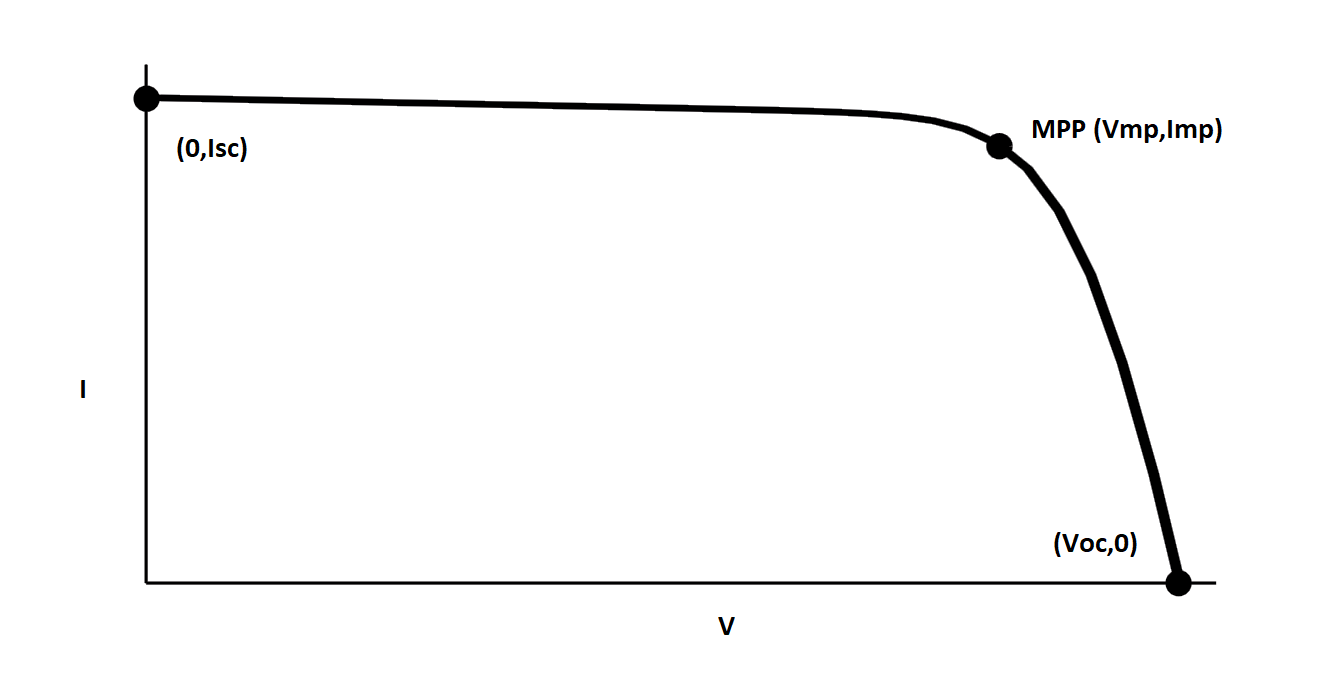
\includegraphics[width=10cm]{figuras/PV.png} 
\label{FigPVprofile}
\end{figure}
\par O modelo do painel solar fotovoltáico está na figura \ref{figPVsim}. Os resistores $R_p$ e $R_s$ podem ser estimados usando metódo interativo presente em \cite{VillalvaRuppert}. O resistor $R_p$ podem tem valor inicial dado por \ref{Rp} e $R_s \approx 0$.
\par Pela figura \ref{FigPVprofile}, nota-se que há um ponto de máxima potência (MPP). Para todos os outros pontos de tensão e corrente, a potência será menor que isso, acarretando perdas de eficiência do conjunto. 
\begin{equation}
    I=I_{pv}-I_o\big[ e^{(\frac{V+R_s.I}{V_t.a})} - 1 \big] - \frac{V+R_s.I}{R_p}
    \label{IPV}
\end{equation}
\begin{equation}
    V_t=\frac{N_s.k.T}{q}
    \label{IPV_Vt}
\end{equation}

\begin{equation}
    Rp_{min}=\frac{V_{mp}}{I_{sc}-I_{mp}} - \frac{V_{oc}-V_{mp}}{I_{mp}}
    \label{Rp}
\end{equation}
\begin{figure}[H]
\caption{Modelo do painel fotovoltáico. Retirada de \cite{VillalvaRuppert}} 
\begin{center}
\begin{circuitikz}
%Coluna,Linha
%(0,0) botton left
\draw
    (0,0)   to [short,-*] (6,0)
    (3.5,4) to [R, i=$I$, l_=$R_s$] (5.5,4)
    (5.5,4) to [short,-*] (6,4)
    (0,0)   to [american current source, l_=$I_{pv}$] (0,4)
    (0,4)   to [short] (3.5,4)
    (1.5,4) to [short, *-, i=$I_d$] (1.5,3) 
    (1.5,3) to [D] (1.5,1)
    (1.5,1) to [short,-*] (1.5,0) 
    (3,4)   to [R, *-*, l_=$R_p$] (3,0); 

\end{circuitikz}
\end{center}
\label{figPVsim}
\end{figure}




\section{Bateria de Íons de Litio}
\par Há vários métodos para carregamento de baterias de Íons de lítio.\cite{YONG2015365}. O método mais convencional e utilizado aqui será com corrente constante/tensão constante, representado na figura \ref{Figbatprofile}. Este método se utiliza de duas etapas: 
\begin{enumerate}
    \item CC - Mantém a corrente constante mesmo que a tensão caia abaixo do valor nominal de carregamento. 
    \item CV - Mantém a tensão constante até o fim do carregamento. 
\end{enumerate}

\begin{figure}[H]
\caption{Perfil de carga de bateria de Íons de litio. Retirada de \cite{YONG2015365}, traduzida pelo autor.}
 \centering % para centralizarmos a figura
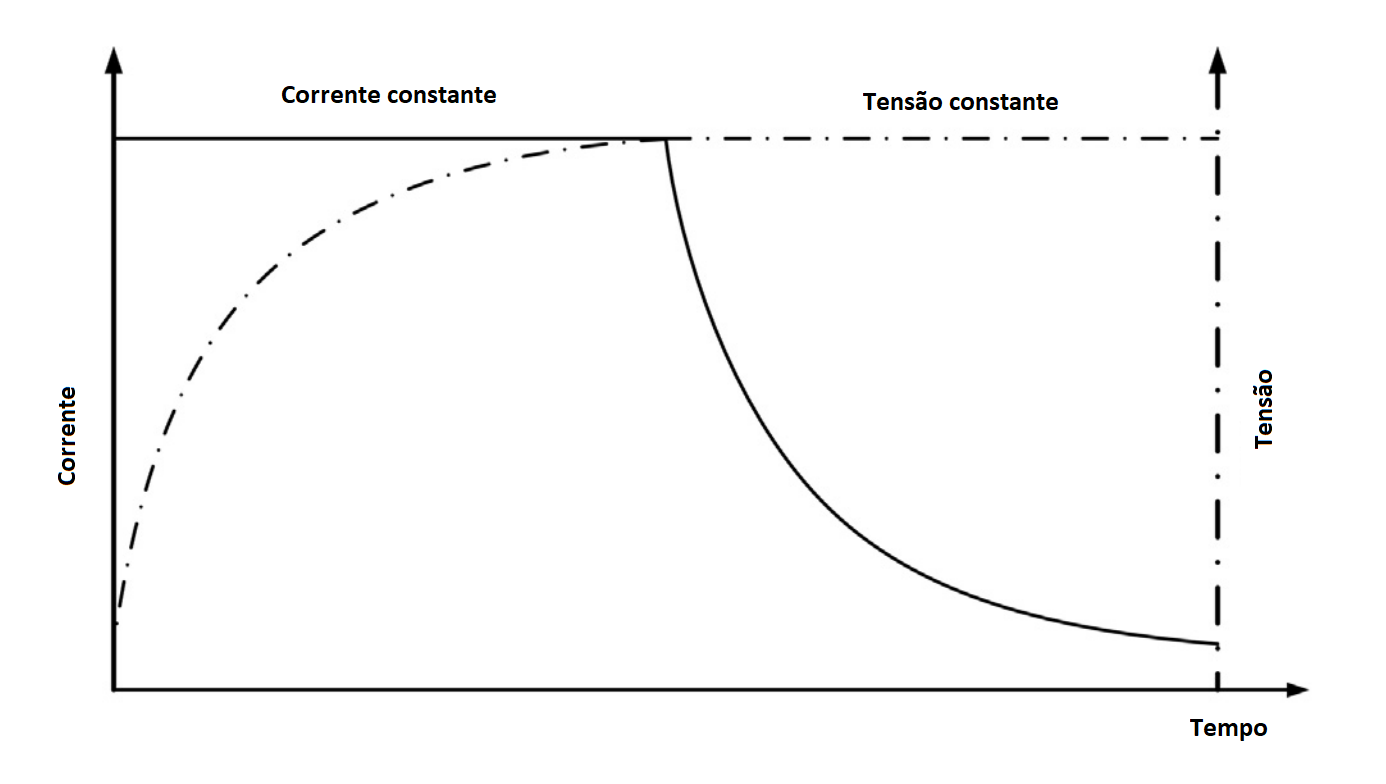
\includegraphics[width=10cm]{figuras/BateriaProfile.png} 
\label{Figbatprofile}
\end{figure}

\chapter{Metodologia utilizada}
\label{chapterMetodologia}
%1. Introdução sobre o sistema que será simulado\\
%2. Diagrama de bloco da pisco de luz\\
%3. MPPT\\
%4. Simulação de Bateria - Estagios de carga de 18650\\
%5. Buck com GAN\\
%%6. interessante não simular controle e sim apenas os 3 pontos importantes de carga: Fonte de corrente, Fonte de tensão\\%
%7. Usar indutor acoplado para amostrar a corrente\\
%0. colocar primeiro: Estudar a relação de beneficios em se utilizar dispositivos GaN ao invés de Silício. Ainda avaliar, se possível, seu custo e viabilidade atuais, no contexto de fontes chaveadas. Especificamente podemos escolher uma topologia simples para base de comparação.
%encontrar nome da descontinuidade no gate do GaN
\par Neste trabalho, toda a análise será fundamentada em simulação computacional utilizando o software LTSpice, da Analog Devices \cite{ltspice}. Os circuitos analisados estão representados na figura \ref{figPVBuckBat} e serão analisados separadamente. \footnote{Os circuitos simulados aqui se encontram disponíveis para download no repositório do autor: \url{www.github.com/phneves/BuckGaN}}

\begin{figure}[H]
\caption{Modelo de simulação completo} 
\begin{center}
\begin{circuitikz}
%Coluna,Linha
%(0,0) botton left
\draw %painel solar
    [dashed] (-1,-1)   to [short,i=] (6,-1)
             (6,-1)   to [short] (6,5)
             (6,5)   to [short] (-1,5)
             (-1,5)   to [short] (-1,-1)
            (3,-0.8) node[]{Painel Solar Fotovoltaico};
\draw %buck
    [dashed] (7,-1)   to [short,i=] (12,-1)
             (12,-1)  to [short] (12,5)
             (12,5)   to [short] (7,5)
             (7,5)   to [short] (7,-1)
            (9.5,-0.8) node[]{Conversor Buck};
\draw %bat
    [dashed] (13,-1)   to [short,i=] (15,-1)
             (15,-1)  to [short] (15,5)
             (15,5)   to [short] (13,5)
             (13,5)   to [short] (13,-1)
             (14,-0.8) node[]{Bateria};
\draw
    (0,0)   to [short,-*] (6,0)
    (3.5,4) to [R, l_=$R_s$] (5.5,4)
    (5.5,4) to [short,-*] (6,4)
    (0,0)   to [american current source, l_=$I_{pv}$] (0,4)
    (0,4)   to [short] (3.5,4)
    (1.5,4) to [short, *-, i=$I_d$] (1.5,3) 
    (1.5,3) to [D] (1.5,1)
    (1.5,1) to [short,-*] (1.5,0) 
    (3,4)   to [R, *-*, l_=$R_p$] (3,0); 
\draw
    %(6,0)   to [short,*-] (7,4)
    %(7,4)   to [short,*-] (8,4)
    (6,4)   to [short,*-] (8,4)
    %(8,4)   to [switch, l_=$GaN$] (10,4)
    (10,4) to[Tnjfet,n=jfet] (8,4)
    %(6,4)   to [short,*-] (7,0)
    %(7,0)   to [short,*-] (14,0)
    (6,0)   to [short,*-] (12,0)
    (12,0)   to [short,*-*] (14,0) 
    (8,0)   to [C,*-*] (8,4)
    (10,0)  to [D,*-*] (10,4)
    (10,4)  to [L,l_=$L$] (12,4) 
    (12,4)   to [short,*-] (14,4) 
    (14,4)  to [battery,-] (14,0)
    node[ground]{};
\end{circuitikz}
\end{center}
\label{figPVBuckBat}
\end{figure}

\section{Conversor Buck}
Considere as topologias apresentadas na na figura \ref{figBuckDiodoGan}. O conversor Buck será analisado em 4 configurações: 1. GaN(EPC2001) + Diodo; 2. 2xGaN; 3. Mosfet(IRF530) + Diodo; 4. 2xMosfet(IRF530).
\begin{figure}[H]
\caption{Model de simulação completo} 
\begin{center}
\begin{circuitikz}
%Coluna,Linha
%(0,0) botton left

\draw
    (0,4)   to [american voltage source, l_=$V_{in}$] (0,0)
    (0.6,4.2) node[]{$V_{in}$}
    (0,4)   to [short,-] (1,4)
    (3,4) to[Tnjfet,n=jfet] (1,4)
    %(6,4)   to [short,*-] (7,0)
    %(7,0)   to [short,*-] (14,0)
    (0,0)   to [short,-] (7,0)
    %(12,0)   to [short,-] (15,0) 
    (1.2,0)   to [C,l_=$C_{in}$, *-*] (1.2,4)
    %(3,0)  to [D,l_=$D$,*-*,color=red] (3,4)
    (3,4)  to [L,l_=$L$,i=$I_o$] (5,4) 
    (5,4)   to [short,-] (7,4) 
    (5.5,4)   to [C,l_=$C_{out}$,*-*] (5.5,0)
    (6,4.2) node[]{$V_{o}$}
    (7,4)  to [R,l_=$R_{o}$,-*] (7,0)
    node[ground]{};
    
    \draw
    (8,4)   to [american voltage source] (8,0)
    (8.6,4.2) node[]{$V_{in}$}
    (8,4)   to [short,-] (9,4)
    (11,4) to[Tnjfet,n=jfet] (9,4)
    %(6,4)   to [short,*-] (7,0)
    %(7,0)   to [short,*-] (14,0)
    (8,0)   to [short,-] (15,0)
    %(12,0)   to [short,-] (15,0) 
    (9.2,0)   to [C, *-*] (9.2,4)
    %(11,0)  to [D,l_=$D$,*-*] (11,4)
    %(11,0) to[Tnjfet,n=jfet,color=red, *-*] (11,4)
    (11,4)  to [L,l_=$L$,i=$I_o$] (13,4) 
    (13,4)   to [short,-] (15,4) 
    (13.5,4)   to [C,l_=$C_{out}$,*-*] (13.5,0)
    (14,4.2) node[]{$V_{o}$}
    (15,4)  to [R,l_=$R_{o}$,-*] (15,0)
    node[ground]{};
    
\draw 
[red] (11,0) to[Tnjfet,n=jfet,color=red, *-*] (11,4)
(3,0)  to [D,l_=$D$,*-*,color=red] (3,4)
;
\end{circuitikz}
\end{center}
\label{figBuckDiodoGan}
\end{figure}
\par Os componentes EPC2001 e IRF530 estão detalhados na tabela \ref{t_ComparaTransistor} \cite{IRF530},\cite{epc2001C}.
\begin{table}[H]
\centering
\caption{Transistores usados nas simulações}
\begin{tabular}{llllll}
\hline
Transistor & $I_d$                     & $V_{gs}$ & $V_{ds}$ & $Rds_{on}$ & $Q_G$  \\ \hline
ECP2001C   & $36A$                     & $5V$  & $100V$                        & $5,6m\Omega $                          & $7.5nC$             \\
IRF530     &  $14A$                      & $5V$  & $100V$                        & $160m\Omega $                          & $26nC$              \\
\hline
\end{tabular}
\label{t_ComparaTransistor}
\end{table}

\par Variando-se a frequência de trabalho, foi calculado os valores dos componentes e \textit{duty-cycle}($\delta$) para cada uma das topologias, seguindo as equações descritas na seção \ref{sectionCap2Buck}. Os valores se encontram na tabela \ref{t_VariacaoFrequencia}.

\begin{table}[H]
\centering
\caption{Valores para conversor Buck variando-se a frequência de trabalho}
\begin{tabular}{llllllllll}
\hline
$f$  &	$V_o$	& $V_{in}$ &	$\delta$	& L & Periodo ($\tau$)	& $I_o$	& $\Delta V_o (mV)$	& $C_o$ & 	Ro($\Omega$)  \\ \hline
$ 25kHz$	& $4,3V$	& $17V$	& $25\%$	& $107\mu H$	& $40 \mu s$& $0,6A$	& $600mV$	& $10\mu F$	& $7,15 \Omega$  \\
$ 50kHz$    & $4,3V$    & $17V$	& $25\%$	& $53,5\mu H$	& $20\mu s$	& $0,6A$	& $300mV$	& $10\mu F$	& $7,15 \Omega$  \\
$100kHz$	& $4,3V$	& $17V$	& $25\%$	& $26,8\mu H$	& $10\mu s$	& $0,6A$	& $150mV$	& $10\mu F$	& $7,15 \Omega$  \\
$200kHz$	& $4,3V$	& $17V$	& $25\%$	& $13,4\mu H$	& $5\mu s$	& $0,6A$	& $75mV$	& $10\mu F$	& $7,15 \Omega$  \\
$300kHz$	& $4,3V$	& $17V$	& $25\%$	& $8,92\mu H$	& $3,33\mu s$& $0,6A$	& $50mV$	& $10\mu F$	& $7,15 \Omega$  \\
$400kHz$	& $4,3V$	& $17V$	& $25\%$	& $6,69\mu H$	& $2,5\mu s$ & $0,6A$	& $37mV$	& $10\mu F$	& $7,15 \Omega$  \\
$500kHz$	& $4,3V$	& $17V$	& $25\%$	& $5,35\mu H$	& $2\mu s$	 & $0,6A$	& $30mV$	& $10\mu F$	& $7,15 \Omega$  \\ \hline
\end{tabular}
\label{t_VariacaoFrequencia}
\end{table}

\par Variando-se a tensão de entrada $V_{in}$, com frequência $f=100kHz$, foi calculado os valores dos componentes e \textit{duty-cycle}($\delta$) para cada uma das topologias, seguindo as equações descritas na seção \ref{sectionCap2Buck}. Os valores se encontram na tabela \ref{t_VariacaoTensao}.

\begin{table}[H]
\centering
\caption{Valores para conversor Buck variando-se a tensão de entrada}
\begin{tabular}{lllllllll}
\hline
$V_{in}$ &	$V_o$	& 	$\delta$ &	L &  $I_o$	& $C_o$ & 	Ro($\Omega$)  \\ \hline
$13V$	& $4,3V$ & $33,07\% $ &  $24\mu H$	& 0,6	& $10 \mu F$	& $7,15 \Omega$ \\
$15V$	& $4,3V$ & $28,66\% $ &  $25,6\mu H$	& 0,6	& $10 \mu F$	& $7,15 \Omega$ \\
$17V$	& $4,3V$ & $25,29\% $ &  $26,8\mu H$	& 0,6	& $10 \mu F$	& $7,15 \Omega$ \\ 
\hline
\end{tabular}
\label{t_VariacaoTensao}
\end{table}

\section{Painel solar fotovoltaico}
\par O Painel solar usado nas simulações foi baseado no circuito da figura \ref{figPVsim} e os resistores $R_s$ e $R_p$ calculados como em \ref{Rp}. Os valores estão presentes na tabela \ref{t_PV}

\begin{table}[H]
\centering
\caption{Valores para o modelo de painel solar fotovoltaico KM(P)10 de 10W}
\begin{tabular}{ll}
\hline
Parâmetro & Valor \\\hline
$V_{mp}$       & $17,56V$                    \\
$I_{sc}$       & $0,66A$                      \\
$I_{mp}$       & $0,6A$                       \\
$V_{oc}$       & $21,52V$                     \\
$R_p$       & $286\Omega$               \\
$R_s$        & $0,01\Omega$                    \\
\hline
\end{tabular}
\label{t_PV}
\end{table}


\chapter{Resultados e conclusões parciais}
\label{chapterResultados}
%mostrar simulação do painel solar\\
%mostrar mppt\\
%mostrar simulação do buck \\
%mostrar simulação do ci LT8491 com e sem gan
%mostrar optmos da infineon se der pra simular o limite de frequência dos transistores e comparar rdson  e frequência 

\section{Conversor Buck}
%grafico de eficiencia por volts de entrada
%Grafico do indutor por frequencia baseado na tabela. 
\par Os transistores do tipo $GaN$ melhoram a eficiência do circuito quando comparados à mesma topologia utilizando transistores de Si. No gráfico da figura \ref{GrafEficienciaFrequencia} é possivel notar que a topologia com transistores $GaN$ é mais eficiente($\approx 3,5\%$ maior) e isso se deve ao $Rds_{on}$ menor, como mostrado na seção \ref{sectionCap2transistores} e na tabela \ref{t_ComparaTransistor}. O mesmo acontece nas altas frequências: o transitor GaN mantém sua performance com poucas perdas, diferentemente dos transistores de Si.  
\par A escolha da topologia tem bastante influência na eficiência global do conversor. Nota-se um grande ganho de eficência em topologias com dois transistores ao inves de um transistor e um diodo. O diodo $D$ dissipa $P=I_d.V_d$, nos momentos em que conduz ($1-\delta$).
\begin{center}
\begin{figure}[H]
\caption{Eficiência em função da frequência.}
\begin{tikzpicture}
\pgfplotsset{
every axis legend/.append style={ at={(1.05,0.95)}, anchor=north west,legend columns = 1}}
\begin{axis}[
  xlabel=Frequencia em $kHz$,
  ylabel=Eficiência em $\%$]
\addplot table [y=G, x=f]{Freq.dat};
\addlegendentry{GaN+diodo}
\addplot table [y=M, x=f]{Freq.dat};
\addlegendentry{Mosfet+diodo}
\addplot table [y=GG, x=f]{Freq.dat};
\addlegendentry{2xGaN}
\addplot table [y=MM, x=f]{Freq.dat};
\addlegendentry{2xMosfet}
\end{axis}
\end{tikzpicture}
\label{GrafEficienciaFrequencia}
\end{figure}
\end{center}
\par Transistores GaN também possibilitam o aumento a frequencia de chaveamento. O benefício direto do aumento da frequencia de trabalho é a diminuição dos elementos magnéticos e portanto, menor custo. Para a fonte estudada neste trabalho, o indutor mínimo ($L_{min}$) está representado na figura \ref{GrafIndutorFrequencia}. Comparando a frequência mais baixa ($25kHz$ ) e a frequência mais alta ($500kHz$), pode-se diminuir de $100\mu  H$ (18,54mm x 15,24mm x 7,11mm) para $5,6\mu H$ (4,7mm x 4,2mm x 3,45mm), além da redução de $\approx 60\%$ no custo médio/componente.
\begin{center}
\begin{figure}[H]
\caption{Eficiência em função da frequência.}
\begin{tikzpicture}
\pgfplotsset{
every axis legend/.append style={ at={(1.05,0.95)}, anchor=north west,legend columns = 1}}
\begin{axis}[
  xlabel=Frequencia em $kHz$,
  ylabel=Indutância em $\mu H$]
\addplot table [y=L, x=f]{L.dat};
\addlegendentry{$V_{in}=17V$; $\delta=25\%$}
\end{axis}
\end{tikzpicture}
\label{GrafIndutorFrequencia}
\end{figure}
\end{center}
\par As simulações também comtemplam a variação da tensão de saída do painel solar fotovoltaico, uma vez que tensão de saída e corrente maxima podem variar de acordo com nível de iluminação disponível. A eficiência em relação à tensão $V_{in}$ está no gráfico da figura \ref{GrafEficienciaTensao}. 
\begin{center}
\begin{figure}[H]
\caption{Eficiência em função da tensão}
\begin{tikzpicture}
\pgfplotsset{
every axis legend/.append style={ at={(1.05,0.95)}, anchor=north west,legend columns = 1}}
\begin{axis}[
  xlabel=Tensão em $V$,
  ylabel=Eficiência em $\%$]
\addplot table [y=GD, x=T]{tensao.dat};
\addlegendentry{GaN+Diodo}
\addplot table [y=MD, x=T]{tensao.dat};
\addlegendentry{Mosfet+Diodo}
\addplot table [y=2G, x=T]{tensao.dat};
\addlegendentry{2xGaN}
\addplot table [y=2M, x=T]{tensao.dat};
\addlegendentry{2xMosfet}
\end{axis}
\end{tikzpicture}
\label{GrafEficienciaTensao}
\end{figure}
\end{center}
\par A tensão de saída das fontes está na figura \ref{fig:BuckVoAll}. Nota-se menor $\Delta V$ nas topologias com frequência maior, e a tensão de saída $V_o$ mais proxima da nominal ($4.3V$) nas topologias com dois diodos, uma vez que o diodo proporciona uma queda de $\approx 0,7V$ (o duty-cycle $\delta$ não foi recalculado para manter a comparação de eficiência). 
\par Os testes até o momento são em \textit{open loop}, com foco em dois parametros: $Rds_{on}$ e frequência.

\begin{figure}[H]
\centering
\caption{Tensão de saída $V_o$, \textit{open loop}, com variação da Frequência e Indutor.}
\subfloat[][GaN+Diodo]{
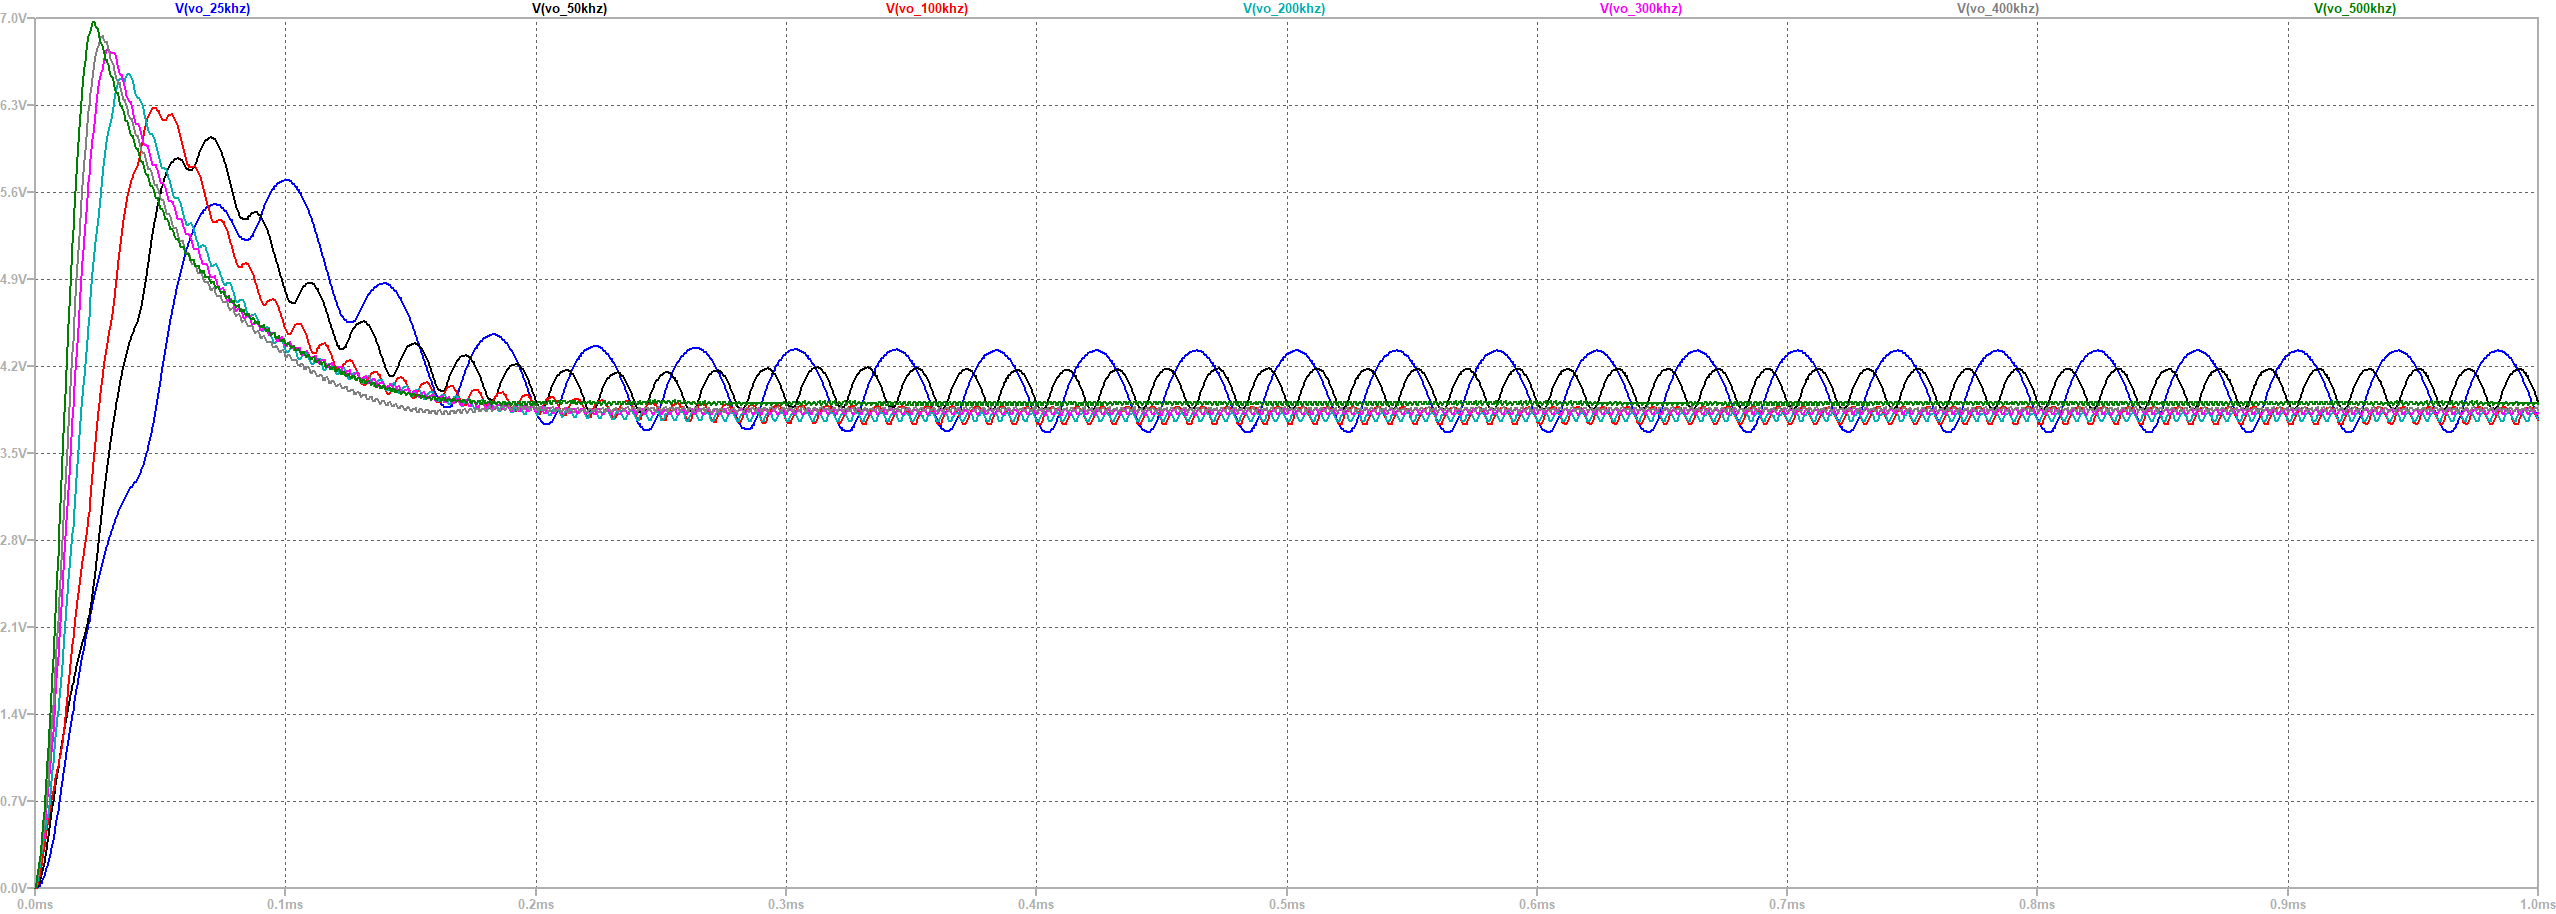
\includegraphics[width=0.5\textwidth]{figuras/Vo_Buck_Gan_Diodo.png} 
\label{fig:subfig1}}
\subfloat[][2xGaN]{
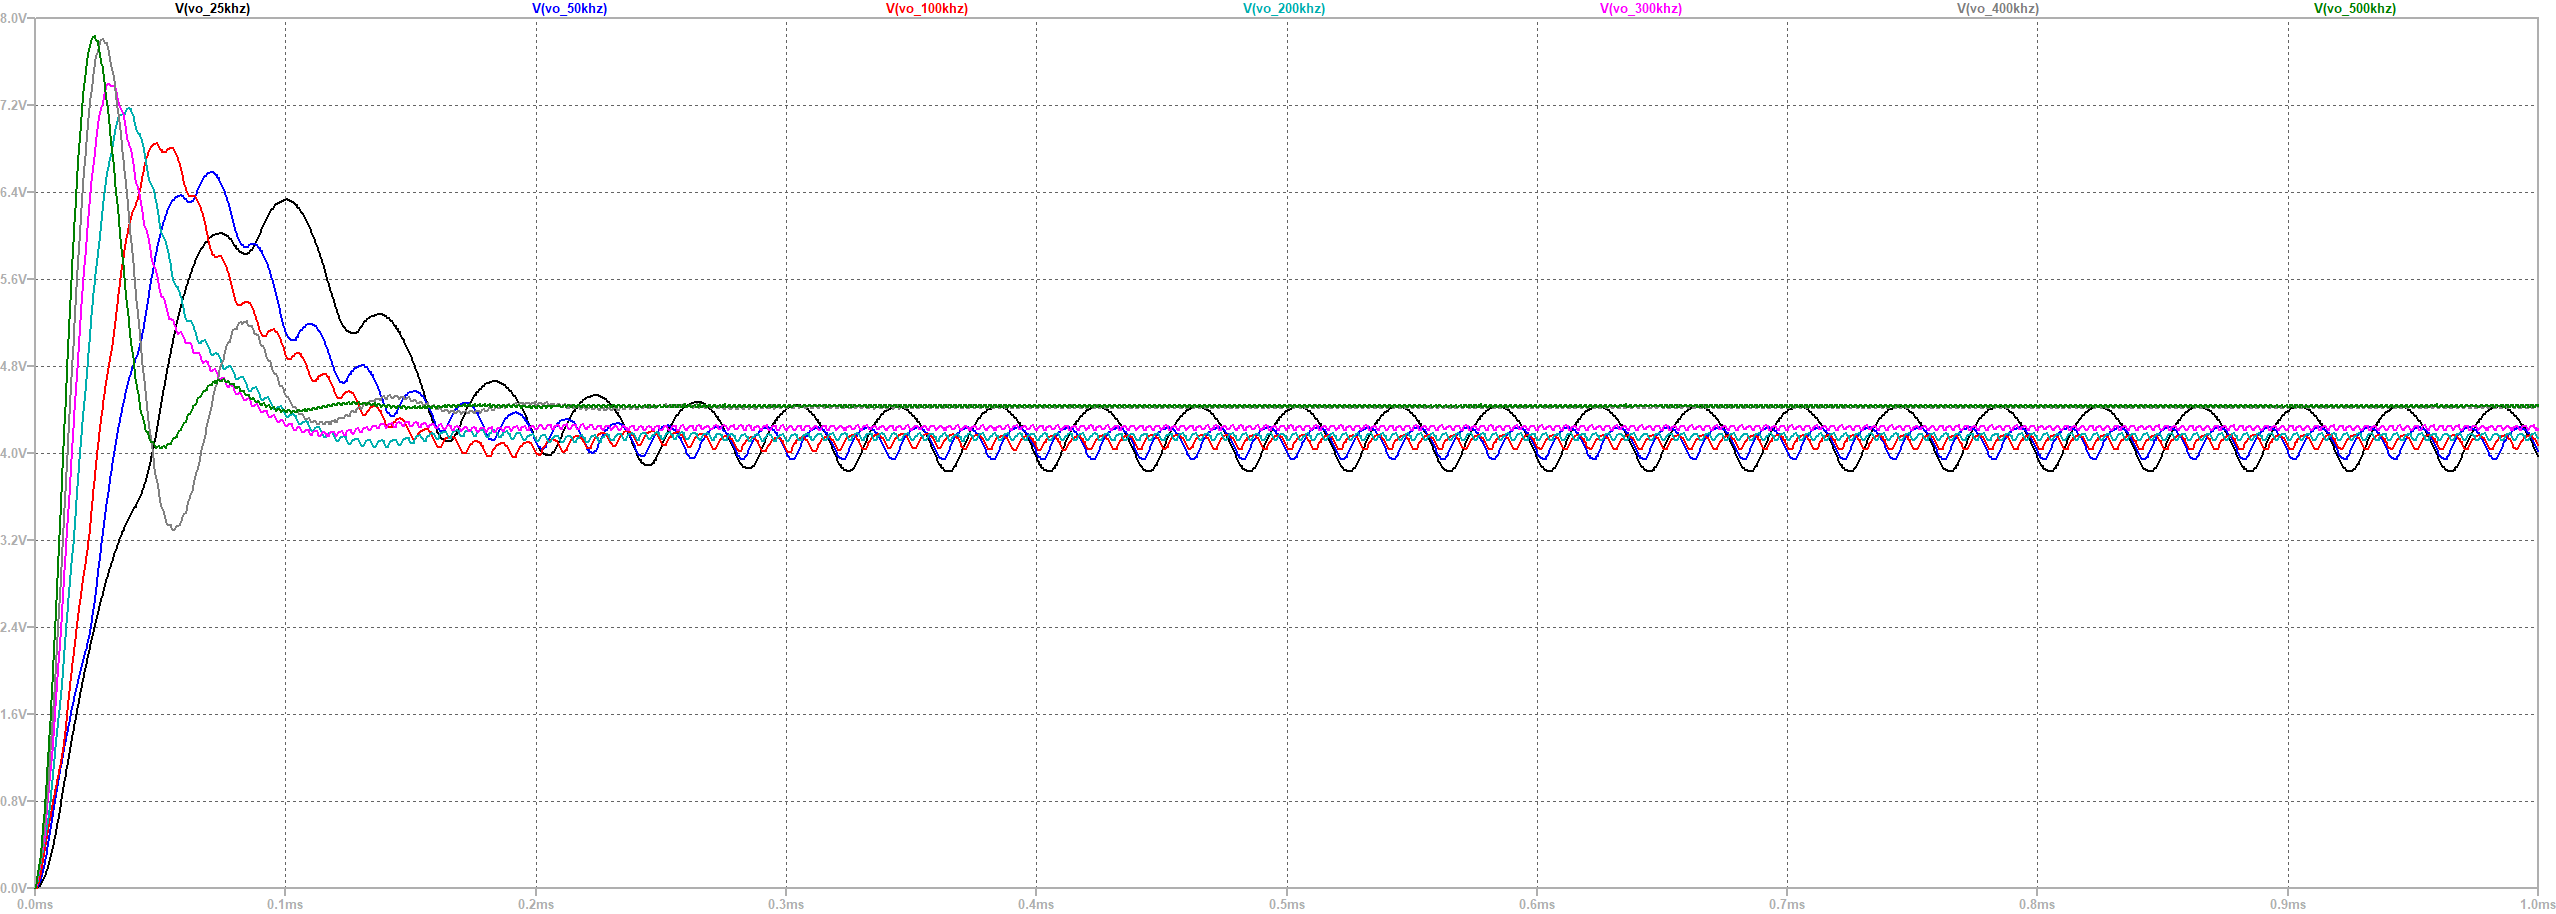
\includegraphics[width=0.5\textwidth]{figuras/Vo_Buck_Gan_Gan.png} 
\label{fig:subfig2}}
\qquad
\subfloat[][Mosfet+Diodo]{
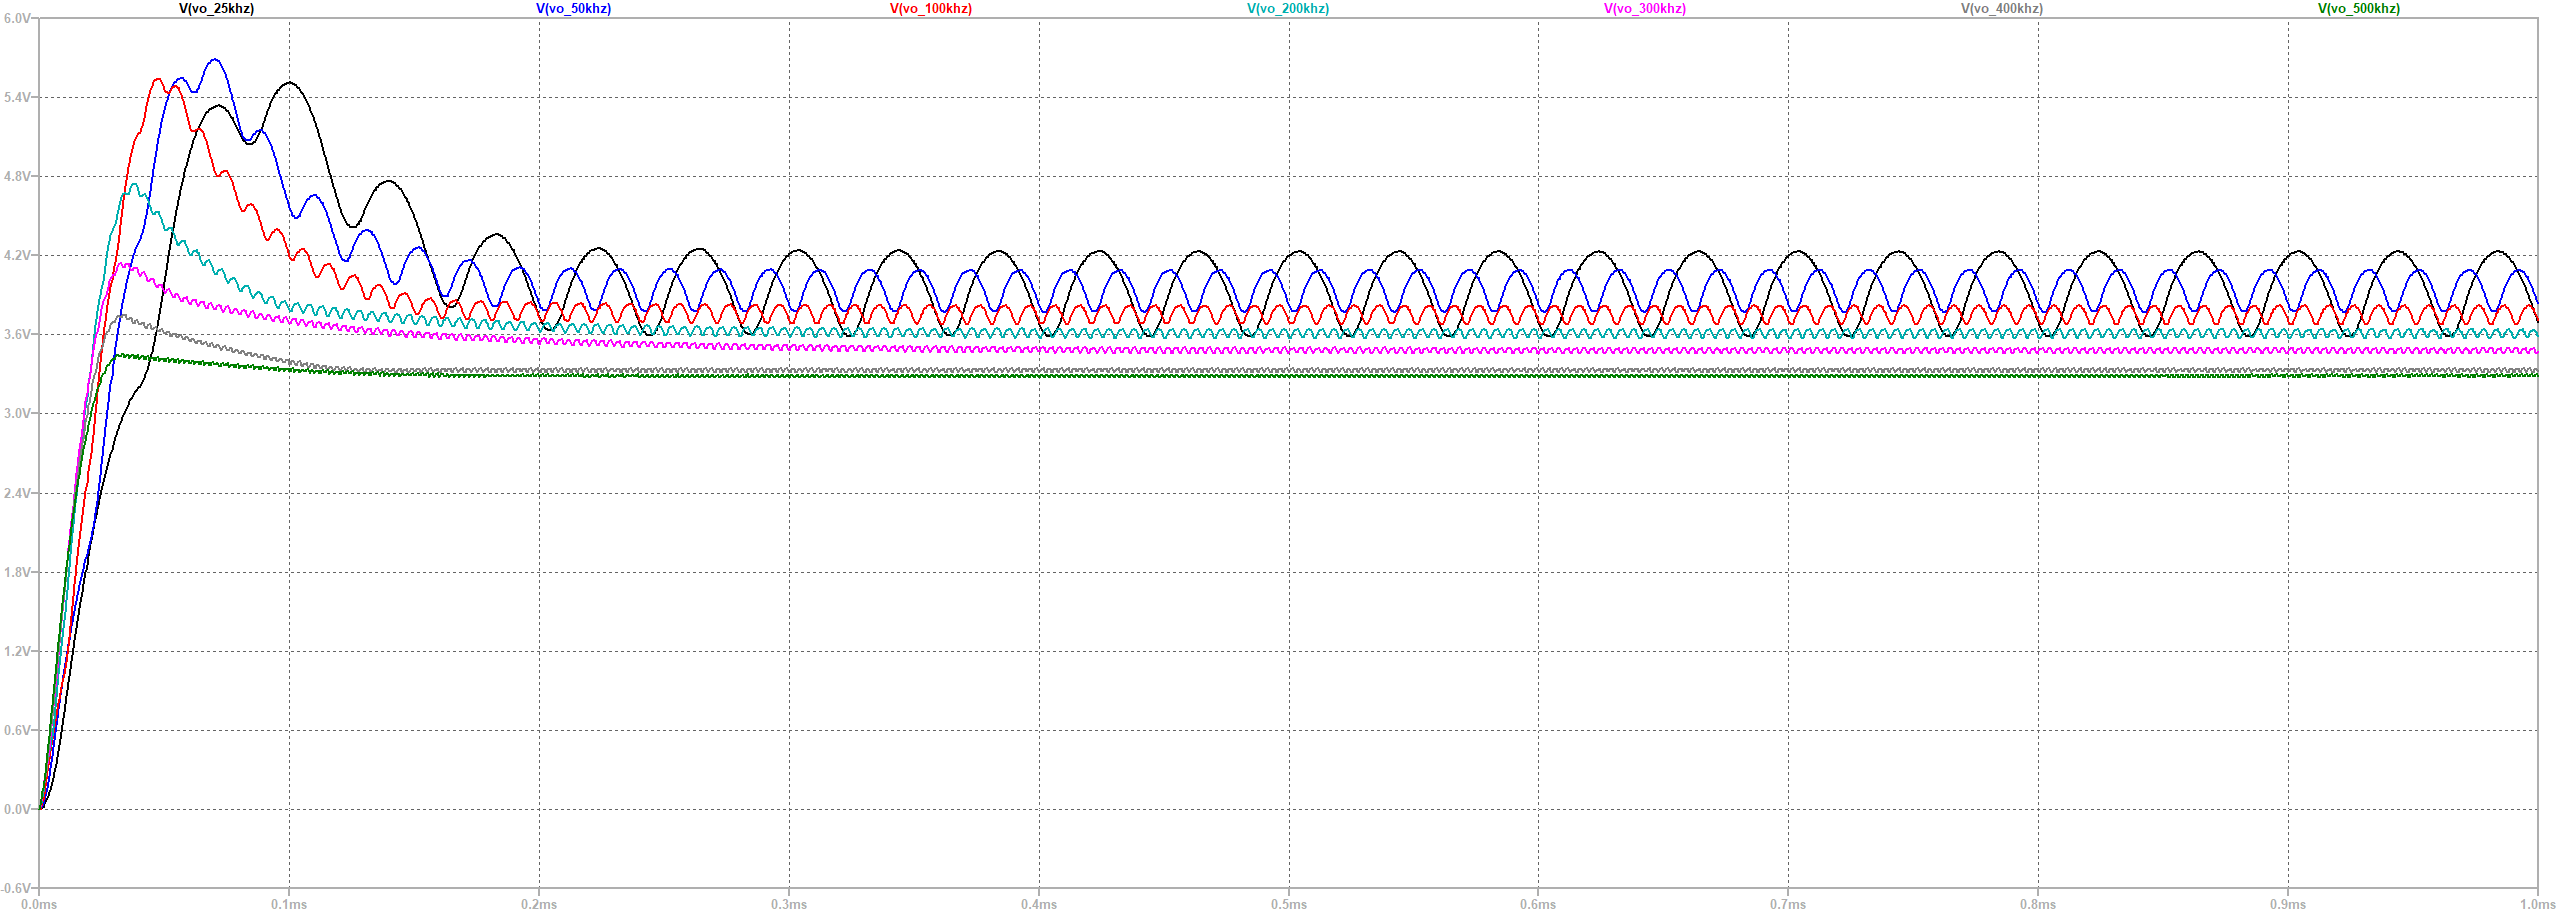
\includegraphics[width=0.5\textwidth]{figuras/Vo_Buck_Mosfet_Diodo.png} 
\label{fig:subfig3}}
\subfloat[][2xMosfet]{
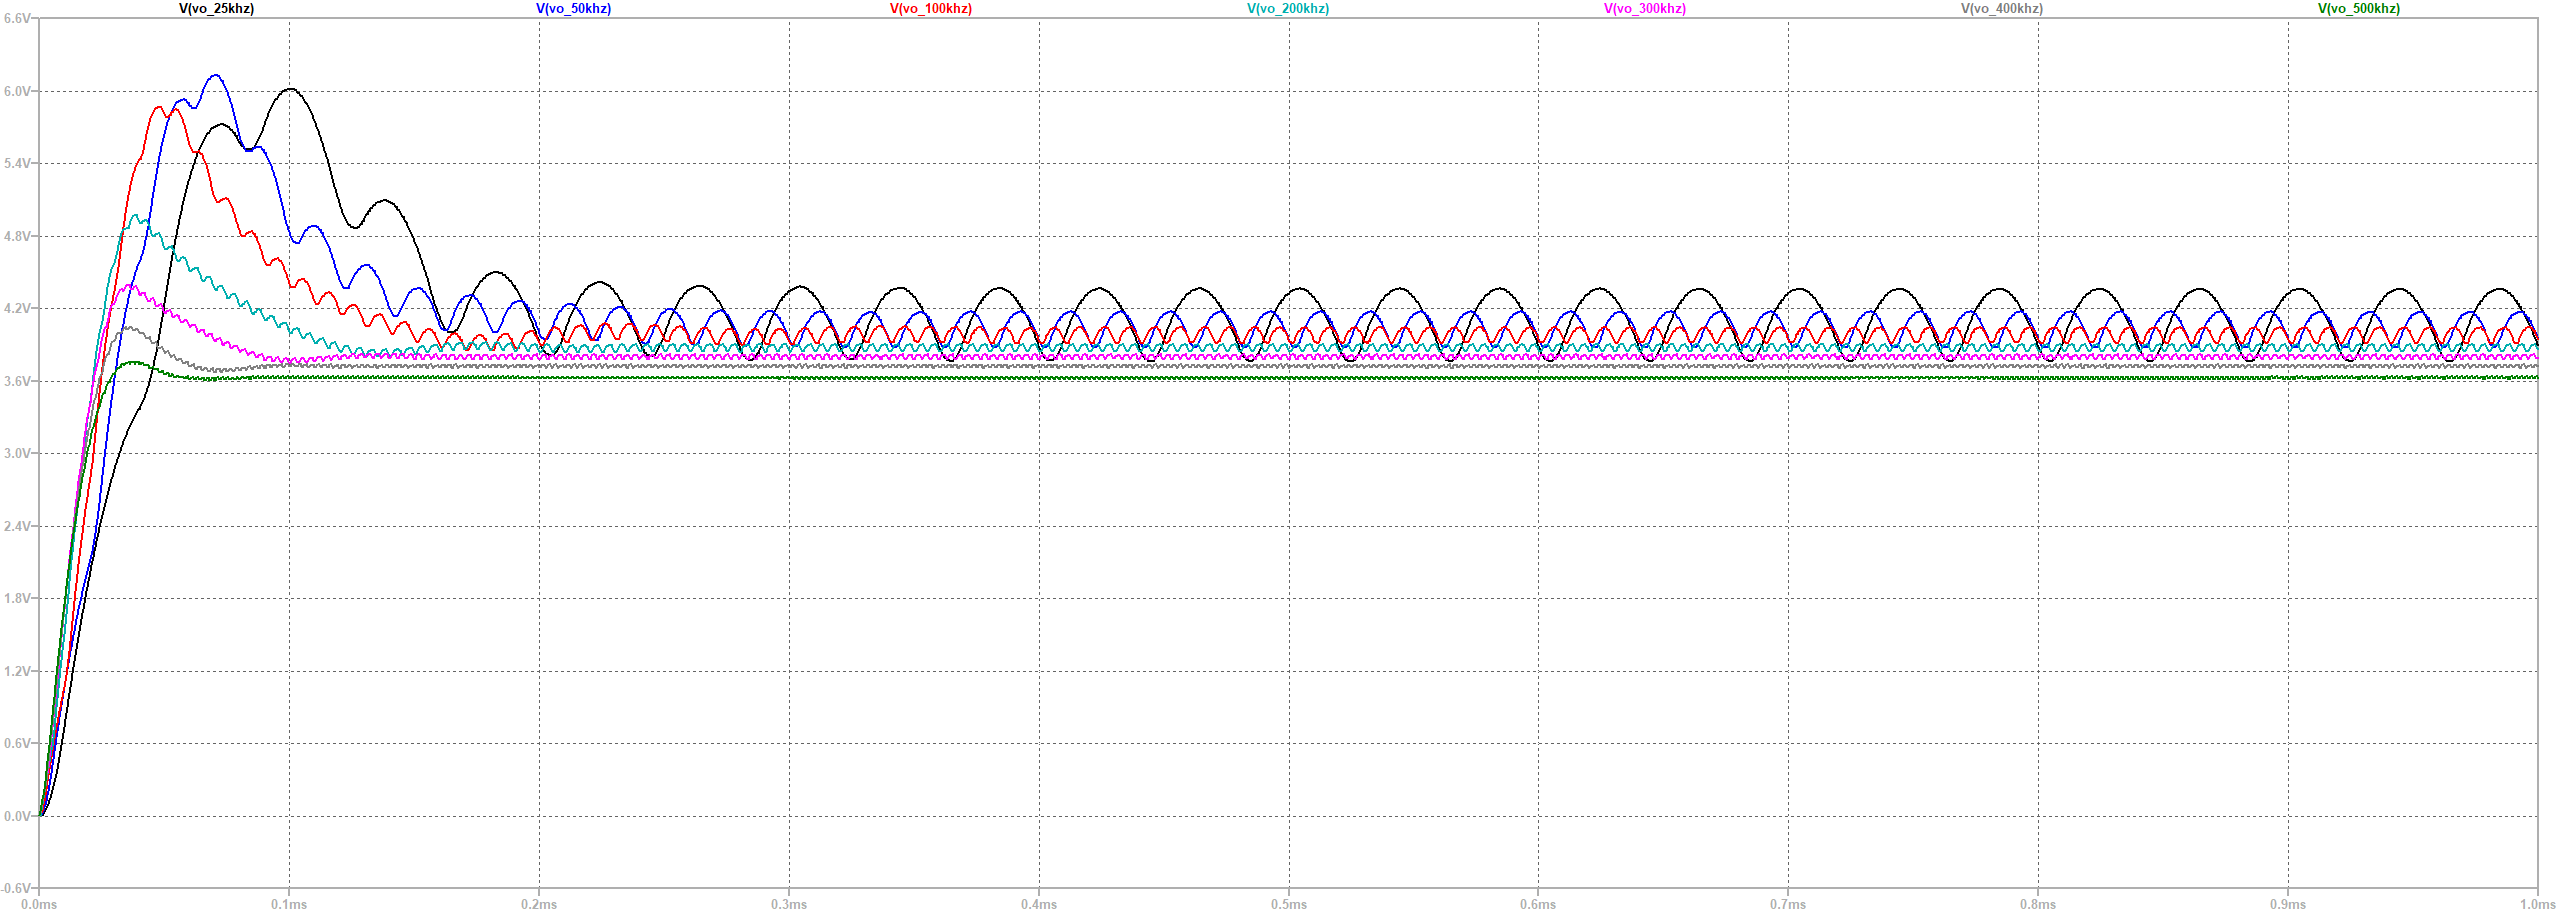
\includegraphics[width=0.5\textwidth]{figuras/Vo_Buck_Mosfet_Mosfet.png} 
\label{fig:subfig4}}
\label{fig:BuckVoAll}
\end{figure}

\section{Painel solar fotovoltaico}
A simulação do Painel solar está representada na figura \ref{FigPV} e pode ser comparada com a tabela \ref{t_PV}. Os parâmetros de Potência máxima($P_{max}=V_m.I_m$) estão bem representados nesta simulação. $V_m \approx 17V$ e $I_{m} \approx 0.6A$ coincidem com $P_{max}$ simulado e o apresentado pelo fabricante.
\par A tensão de circuito aberto ($V_{oc}$) não está representada adequadamente e deve sofrer reajustes no modelo.
\begin{figure}[H]
\caption{Simulação painel solar fotovoltáico}
 \centering % para centralizarmos a figura
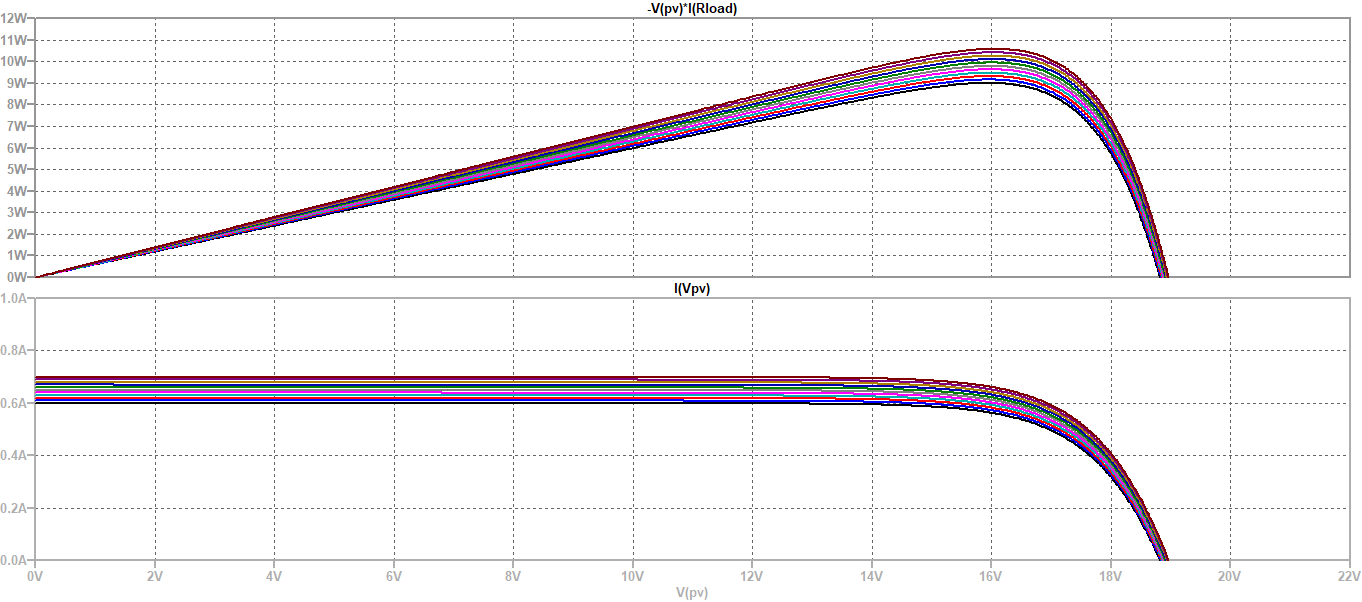
\includegraphics[width=14cm]{figuras/PV_resultados.png} 
\label{FigPV}
\end{figure}

\chapter{Plano de trabalho e cronograma}
\label{chapterCronograma}
\par Paragrafo explicando o cronograma.
%adicionar algum comentario sobre a linha do tempo
\begin{figure}[H]
\caption{Cronograma} 
\begin{center}
\begin{circuitikz}
%draw horizontal line
\draw (0,0) -- (14,0);
\draw [dashed](14,0) -- (15,0);
%draw vertical lines
\foreach \x in {0,1,3,5,7,10.5,14}
\draw (\x cm,3pt) -- (\x cm,-3pt);

%draw nodes
\draw (0,0) node[below=3pt] {$ 2020 $} node[above=3pt] {$   $};
\draw (1,0) node[below=3pt] {$  $} node[above=3pt] {$ I $};
\draw (2,0) node[below=3pt] {$  $} node[above=3pt] {$  $};
\draw (3,0) node[below=3pt] {$  $} node[above=3pt] {$ II $};
\draw (4,0) node[below=3pt] {$  $} node[above=3pt] {$  $};
\draw (5,0) node[below=3pt] {$  $} node[above=3pt] {$  $};
\draw (6,0) node[below=3pt] {$  $} node[above=3pt] {$  $};
\draw (7,0) node[below=3pt] {$ 2021 $} node[above=3pt] {$ III $};
\draw (10.5,0) node[below=3pt] {$ 07/2021 $} node[above=3pt] {$ IV $};
\draw (14,0) node[below=3pt] {$ 2022 $} node[above=3pt] {$ V $};
\end{circuitikz}
\end{center}
\label{figCronograma}
\end{figure}

\par O cronograma da figura \ref{figCronograma} está detalhado a seguir:
\renewcommand{\labelenumi}{\Roman{enumi}}
 \begin{enumerate}
   \item Início do programa
   \item Disciplinas:
    \begin{itemize}
        \item IT505 - Fontes chaveadas
        \item IE320 - Tópicos em Eletrônica I: Introdução a compatibilidade eletromagnética
        \item IT302 - Eletronica de potência I
        \item IT306 - Tópicos em Sistemas de Energia Elétrica III
    \end{itemize}
   \item Inicio das simulações e validações de modelos
   \item Qualificação
   \item Integração dos modelos simulados e apresentação da dissertação

 \end{enumerate}
 


%\chapter{Introdu\c{c}\~ao}
Segundo a \textit{World Semiconductor Trade Statistics}, cada pessoa no planeta comprou uma média de 111 chips ou circuitos integrados (ICs) em 2016. O uso desses dispositivos semicondutores está crescendo cinco vezes a taxa de crescimento da população humana \cite{Sameer}. \par
\noindent Natural que haja uma busca por dispositivos que possibilitem maior densidade de transistores, bem como menor dissipação de energia na forma de calor. Transistores de Nitreto de Gálio e Carbeto de Silício vem se mostrando como alternativa ao cenário atual, com Silício. São bons chaveadores em alta frequência além baixa resistência quando ligados \cite{lidow_rooij_strydom_reusch_glaser_2020}. 

\section{Energia renovavel - Solar}
Intro
\subsection{Pisco de Luz}
Falar sobre a organização. 
\subsection{Sistema de iluminação}

\section{Transistores em circuitos de potência}
\subsection{Transistores de potência baseados em Silício}
Os transistores de potência baseados em silício, tiveram sua eficiência e o custo do gerenciamento de energia melhorado continuamente nas ultimas decadas. Inovações em estruturas do transistor acompanharam a crescente necessidade de equipamentos eletrônicos em nossas vidas diárias. No entanto, a taxa de melhoria diminuiu bastante, uma vez que ,assintoticamente, se aproxima de seus limites teóricos. \cite{lidow_rooij_strydom_reusch_glaser_2020}

\subsection{Transistor baseados em Nitreto de Gálio (GaN)}
Dispositivos baseados em Nitreto de Gálio (GaN) apareceram pela primeira vez em cerca de 2004, como transistores de radiofrequência (RF) feitos pela Eudyna Corporation do Japão. Usando GaN em substratos de carbeto de silício (SiC), a Eudyna produziu transistores projetados para o mercado de RF, com sucesso \cite{Alex}. Porém, não só do ponto de vista de RF há vantagens em utilizar GaN, há vantagens também em eletrônica de potência. As caracteristicas dos dispositivos baseados em Nitreto de Gálio podem ser vistas na comparação da Tabela \ref{t_materiais}.

\begin{table}[!htb]
\centering
\caption{Comparação entre propriedades dos materiais \cite{lidow_rooij_strydom_reusch_glaser_2020}}
\begin{tabular}{lllll}
\hline
Parâmetro           &                & Si    & SiC   & GaN \\ \hline
Banda de Gap $E_g$& $(eV)$             & 1,12  & 3,39  & 3,26\\
Campo Elétrico crítico $E_{Crit}$ &$(MV/cm)$   & 0,23  & 3,3   & 2,2\\
Mobilidade dos elétrons $\mu_n$ &$(cm^2/V.s)$& 1400  & 1500  & 950\\
Permissividade $\varepsilon_r$ &     & 11,8  & 9     & 9,7\\
Condutividade térmica $\lambda$& $(W/cm.K)$     & 1,5   & 1,3   & 3,8\\ \hline
\end{tabular}
\label{t_materiais}
\end{table}

\subsubsection{Banda de Gap $(E_g)$}
A banda de Gap de um semicondutor está relacionado à força das ligações químicas entre os átomos na rede. Essas ligações mais fortes significam que é mais difícil para um elétron saltar de um nível para o próximo. Entre as muitas consequências estão correntes de fuga intrínsecas mais baixas e maiores temperaturas de operação para semicondutores de gap maior. Com base nos dados da Tabela \ref{t_materiais}, GaN e SiC têm banda de Gap maiores do que o silício. \cite{lidow_rooij_strydom_reusch_glaser_2020}

\subsubsection{Resistência quando ligado $(R_{DS_{(on)}})$}
A resistência teórica, em Ohms ($\Omega$), será dada pela equação \ref{RdsOn}. \cite{lidow_rooij_strydom_reusch_glaser_2020}
\begin{equation}
    R_{DS_{(on)}} = \frac{W_{drift}}{q.\mu_n .N_D}
    \label{RdsOn}
\end{equation}
A resistência, quando relacionada com o Campo Elétrico Crítico $(E_g)$ será dada por \ref{RdsOnEg}. \cite{lidow_rooij_strydom_reusch_glaser_2020}
\begin{equation}
    R_{DS_{(on)}} = \frac{4.V^2_{BR}}{\varepsilon_o .\varepsilon_r . E^3_{crit}}
    \label{RdsOnEg}
\end{equation}
A equação dada por \ref{RdsOnEg} está representada no gráfico da Figura \ref{FigRDSon}.
\begin{figure}[H]
\caption{Resistência $R_{DS_(on)}$ vs capacidade de bloquear tensão para dispositivos Si, SiC, and GaN \cite{lidow_rooij_strydom_reusch_glaser_2020}}
 \centering % para centralizarmos a figura
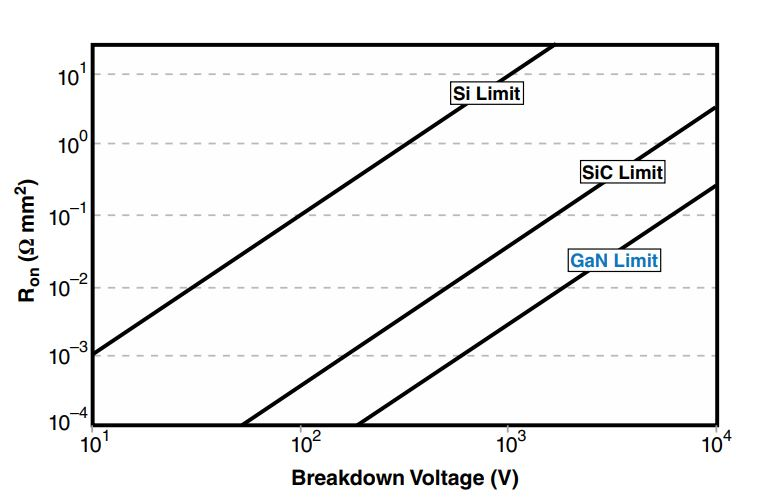
\includegraphics[width=14cm]{figuras/5.JPG} 
\label{FigRDSon}
\end{figure}
\noindent Junto com a baixa resistência $R_{DS_(on)}$, há o benefício de conseguir trabalhar em frequências mais altas que IGBTs com potências relativamente altas, como mostra a Figura \ref{FigComparison}. 
\begin{figure}[H]
\caption{Potência vs Frequência. \cite{Sameer}}
 \centering % para centralizarmos a figura
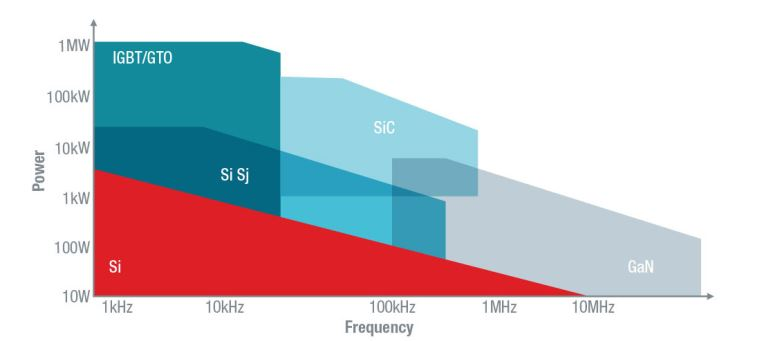
\includegraphics[width=15cm]{figuras/6.JPG} 
\label{FigComparison}
\end{figure}







%\chapter{Objetivos d trabalho}
1. Introdução sobre o sistema que será simulado\\
2. Diagrama de bloco da pisco de luz\\
3. MPPT\\
4. Simulação de Bateria - Estagios de carga de 18650\\
5. Buck com GAN\\
6. interessante não simular controle e sim apenas os 3 pontos importantes de carga: Fonte de corrente, Fonte de tensão\\
7. Usar indutor acoplado para amostrar a corrente\\
0. colocar primeiro: Estudar a relação de beneficios em se utilizar dispositivos GaN ao invés de Silício. Ainda avaliar, se possível, seu custo e viabilidade atuais, no contexto de fontes chaveadas. Especificamente podemos escolher uma topologia simples para base de comparação.

\begin{center}
\begin{circuitikz}
%Coluna,Linha
%(0,0) botton left
\draw %painel solar
    [dashed] (-1,-1)   to [short,i=] (6,-1)
             (6,-1)   to [short] (6,5)
             (6,5)   to [short] (-1,5)
             (-1,5)   to [short] (-1,-1)
            (3,-0.8) node[]{Painel Solar Fotovoltaico}
;

\draw %buck
    [dashed] (7,-1)   to [short,i=] (12,-1)
             (12,-1)  to [short] (12,5)
             (12,5)   to [short] (7,5)
             (7,5)   to [short] (7,-1)
            (9.5,-0.8) node[]{Conversor Buck}
;

\draw %bat
    [dashed] (13,-1)   to [short,i=] (15,-1)
             (15,-1)  to [short] (15,5)
             (15,5)   to [short] (13,5)
             (13,5)   to [short] (13,-1)
             (14,-0.8) node[]{Bateria}
;


        

    
\draw
    (0,0)   to [short,-*] (6,0)
    (3.5,4) to [R, l_=$R_s$] (5.5,4)
    (5.5,4) to [short,-*] (6,4)
    (0,0)   to [american current source, l_=$I_{pv}$] (0,4)
    (0,4)   to [short] (3.5,4)
    (1.5,4) to [short, *-, i=$I_d$] (1.5,3) 
    (1.5,3) to [D] (1.5,1)
    (1.5,1) to [short,-*] (1.5,0) 
    (3,4)   to [R, *-*, l_=$R_p$] (3,0)
    ; 
\draw
    %(6,0)   to [short,*-] (7,4)
    %(7,4)   to [short,*-] (8,4)
    (6,4)   to [short,*-] (8,4)
    (8,4)   to [switch, l_=$GAN$] (10,4)
    %(6,4)   to [short,*-] (7,0)
    %(7,0)   to [short,*-] (14,0)
    (6,0)   to [short,*-] (12,0)
    (12,0)   to [short,*-*] (14,0) 
    (8,0)   to [C,*-*] (8,4)
    (10,0)  to [D,*-*] (10,4)
    (10,4)  to [L,l_=$L$] (12,4) 
    (12,4)   to [short,*-] (14,4) 
    (14,4)  to [battery,-] (14,0)
    node[ground]{}
;
    
\end{circuitikz}
\end{center}



\section{Fonte chaveada de referência}
O objetivo é comparar as propriedades dos dispositivos e como eles afetam uma dada fonte chaveada de referência. O controle da fonte deverá permanecer o mesmo durante a comparação ou até mesmo não ser utilizado. Pode-se analisar a fonte apenas com carga resistiva e em regime permanente. Como exemplo, utilizei um circuito elevador de tensão (boost) bastante simples e sem controle. O circuito está na Figura \ref{FigCircuit} e foi simulado no LTSpice, da Analog Devices \cite{ltspice}.
\begin{figure}[H]
\caption{Circuito de referência: Boost}
 \centering % para centralizarmos a figura
\includegraphics[width=14cm]{figuras/1.JPG} 
\label{FigCircuit}
\end{figure}
\noindent O circuito superior da Figura \ref{FigCircuit} utiliza uma chave simples no lugar de um transistor, com $R_{DS_{(on)}}$ de um transistor GaN comercial. O circuito da parte de baixo da mesma figura, utiliza um $R_{DS_{(on)}}$ de um transistor Mosfet baseado em Silício.\par
\noindent Na figura \ref{FigCircuitVoutIout}, temos a saída dos dois circuitos, $V_{(out)}$ e $I_{(out)}$. Nota-se um grande \textit{overshoot}, dado que não há controle.
\begin{figure}[H]
\caption{Circuito de referência: Tensões e correntes de saída}
 \centering % para centralizarmos a figura
\includegraphics[width=14cm]{figuras/2.JPG} 
\label{FigCircuitVoutIout}
\end{figure}
\noindent Pode-se, então, comparar os rendimentos dos circuitos, baseados apenas nessa característica, $R_{DS_{(on)}}$. Na Figura \ref{FigCircuitEff}, há o calculo feito pelo software. 
\begin{figure}[H]
\caption{Circuito de referência: Comparação da eficiência}
 \centering % para centralizarmos a figura
\includegraphics[width=8cm]{figuras/3.JPG} 
\label{FigCircuitEff}
\end{figure}
\noindent A eficiência desse \textit{Boost} utilizado GaN é de $91,607\%$, enquanto com Silício é de $90,67\%$. Embora pareça pouco a diferença de $~1\%$, deve-se notar que este é um circuito elevador de $5V$ para $10V$, com corrente $I_o$ médio de apenas $0,5A$. Para escalas maiores de potência, $kW$ ou até $MW$, as perdas serão muito maiores.

\section{Oportunidades de publicação}
As pesquisas feitas através do site da IEEE (Journals: \textit{IEEE Transactions on Power Electronics} e \textit{IEEE Journal of Emerging and Selected Topics in Power Electronics}) mostraram que GaN é um tópico que vem crescendo ao longo dos anos, porém ainda com pouco número de publicações. No grafico da Figura \ref{FigPublications}, há o número de publicações, por ano, no IEEE, nos \textit{journals} citados acima. Na revista da Sobraep só foram encontrados dois artigos sobre o tema. 
\begin{figure}[H]
\caption{Número de publicações com os termos "GaN Hemt", por ano}
 \centering % para centralizarmos a figura
\includegraphics[width=14cm]{figuras/IEEE_Graf.JPG}
\label{FigPublications}
\end{figure}
\noindent O número crescente de publicações, indica que o interesse nesse tipo de dispositivo semicondutor cresce na mesma medida. Alguns artigos servirão de norte para este projeto: \cite{Chu}, \cite{Huang}, \cite{mitova}.




%\chapter{Plano de desenvolvimento}

\section{Solução}
Desenvolvimento teórico da solução
simulação da topologia proposta
\section{Oportunidades de publicação}




\section{qualificação}


\section{Artigo}
-Como avaliar rapidamente se vale a pena a adoção de wide gap transitores? 
-quais são as perdas: https://www.infineon.com/dgdl/Infineon-Technical_paper_perspective_of_loss_mechanism_for_silicon_and_wide_band-gap_power_devices-Article-v01_00-EN.pdf?fileId=5546d4625f91ce3d015f91ce8e4d0042

%\chapter{Cronograma}

A ser definido.

%\include{ex5}
%\include{ex6}

% Os comandos para incluir as referências bibliográficas
\begin{singlespacing}
\setlength\bibitemsep{10pt}   % Adiciona uma linha em branco entre duas referências
\printbibliography[heading=bibintoc, % Adiciona no sumário
                   title={Referências bibliográficas} % Nome do Capítulo
                  ]
\end{singlespacing}

% Os anexos, se houver, vêm depois das referências:
%\appendix

% O comando a seguir inclui o arquivo apendices.tex
% que contém os apêndices. Observe o comando \appendix
% na linha anterior
% Detalhe: não precisa incluir a extensão .tex
%\include{apendices}

\end{document}